\documentclass{article}

\usepackage{PRIMEarxiv}

\usepackage[utf8]{inputenc} % allow utf-8 input
\usepackage[T1]{fontenc}    % use 8-bit T1 fonts
\usepackage{hyperref}       % hyperlinks
\usepackage{url}            % simple URL typesetting
\usepackage{booktabs}       % professional-quality tables
\usepackage{multirow}       % multi-row cells in tables
\usepackage{makecell}       % \makecell for stacked cells
\usepackage{placeins}       % \FloatBarrier
\usepackage{float}         % [H] placement specifier
\usepackage{amsfonts}       % blackboard math symbols
\usepackage{nicefrac}       % compact symbols for 1/2, etc.
\usepackage{microtype}      % microtypography
%\usepackage{lipsum} % removed for submission
\usepackage{fancyhdr}       % header
\usepackage{graphicx}       % graphics
\graphicspath{{./}}         % all figures co-located with the .tex for portable Overleaf upload
\usepackage[authoryear]{natbib}
\usepackage{amsmath}

\usepackage{setspace}

\usepackage{xargs}                      % Use more than one optional parameter in a new commands
\usepackage[pdftex,dvipsnames,table]{xcolor}  % Coloured text etc.
\usepackage{colortbl}          % row/cell colors in tables
%\usepackage[disable]{todonotes} % [disable] hides all \todo{} notes for clean PDF; switch to [colorinlistoftodos,prependcaption,textsize=small] while drafting

%\pgfplotsset{compat=1.18}




%Header
\pagestyle{fancy}
\thispagestyle{empty}
\rhead{ \textit{ }} 

% Update your Headers here
\fancyhead[LO]{Distribution-Independent TSP Estimator for Arbitrary Dimension}
% \fancyhead[RE]{Firstauthor and Secondauthor} % Firstauthor et al. if more than 2 - must use \documentclass[twoside]{article}
\usepackage{xcolor}



  
%% Title
\title{Distribution-Independent Estimator for the Traveling Salesman Problem on Arbitrary Dimensions
%%%% Cite as
%%%% Update your official citation here when published 
%\thanks{\textit{\underline{Citation}}: 
%\textbf{Authors. Title. Pages.... DOI:000000/11111.}} 
}

\author{
  Stephen Feldman, James P. Bailey, Bahar \c{C}avdar \\
  Rensselaer Polytechnic Institute, Troy, NY\\
  \texttt{\{feldms5, bailej6, cavdab2\}@rpi.edu} \\
  %% examples of more authors
  % \And
  %Author3 \\
  %Affiliation \\
  %Univ \\
  %City\\
  %\texttt{email@email} \\
  %% \AND
  %% Coauthor \\
  %% Affiliation \\
  %% Address \\
  %% \texttt{email} \\
  %% \And
  %% Coauthor \\
  %% Affiliation \\
  %% Address \\
  %% \texttt{email} \\
  %% \And
  %% Coauthor \\
  %% Affiliation \\
  %% Address \\
  %% \texttt{email} \\
}


\begin{document}
\maketitle


\begin{abstract}
We present Geometrically Assisted Regression Tree (GART) 2.0, a distribution-independent estimator of optimal Traveling Salesman Problem (TSP) tour length whose feature set scales to high dimensions. Existing estimators either require knowledge of the underlying distribution or are not scalable to high dimensions. GART 2.0 is a LightGBM regressor that predicts a scaling ratio $\alpha$, the relationship between the length of the minimum spanning tree and the optimal tour length. We benchmark GART 2.0 against its predecessor and other tour-length estimators from the literature across three datasets. Benchmarking demonstrates that GART 2.0 outperforms the surveyed models while remaining computationally tractable. Because its features scale well with dimension, GART 2.0 can also predict tour lengths for non-Euclidean data. Using multidimensional scaling, the model processes non-Euclidean TSPLIB95 instances translated to high-dimensional Euclidean spaces and makes high-quality estimates. Our results demonstrate that the GART framework can be applied to real-world problems.
\end{abstract}


% keywords can be removed
\keywords{Traveling Salesman Problem\and Tour length estimation \and Distribution-independent \and Multidimensional network}



\onehalfspacing

\section{Introduction}\label{sec:intro}

The Traveling Salesman Problem (TSP) is a fundamental problem in combinatorial optimization, widely used for logistics operations planning, network design, and resource allocation \citep{chien1992operational, concorde2006}. Because determining exact solutions for large-scale instances is NP-hard \citep{karp1972, papadimitriou1977}, the ability to compute rapid tour-cost estimates is essential for real-time decision-making in applications where a full solve is impractical. Tour-cost estimates also serve as inputs to other optimization problems where the TSP appears as a subproblem. For example, in the mobile facility location problem \citep{halper2011mobile}, the objective function includes the cost of a TSP route through customer locations.

\subsection{Background and Motivation}

Tour-length estimation is a key input to strategic logistics decisions where solving the TSP exactly is unnecessary or infeasible. Last-mile delivery accounts for approximately 53\% of total shipping costs \citep{finmile2025}, and the UPS ORION system is reported to save roughly 100 million miles and \$300--400 million annually through route optimization \citep{holland2017ups}. As an extension of the Vehicle Routing Problem (VRP), last-mile delivery solvers use complex heuristics to construct efficient routes. In such systems, recalculation occurs frequently as new orders are added to the system, and the number of customers served by a route is high. Distributors are looking for operational solutions that offer efficient routes without the computational expense of traditional solves. Tour length estimators enable significant computational improvements without sacrificing accuracy.

Beyond traditional logistics, fast TSP length approximation is a critical component across diverse applications in which TSP-like structures arise as subproblems. In bioinformatics, the ordering of markers in radiation hybrid mapping is modeled as a TSP, where rapid cost estimation enables evaluation of assembly quality without full reconstruction \citep{agarwala2000fast}. In data compression, vector quantization partitions a codebook into clusters and must order codewords to minimize transition costs, a problem reducible to TSP on a high-dimensional distance matrix. Additionally, in sensor network design, estimating the minimum data collection path length is crucial for optimizing the lifespan of battery-constrained mobile sinks in wireless sensor networks \citep{wang2008}.

In these domains, the problem is rarely confined to 2D Euclidean space. Genome assembly operates in abstract metric spaces defined by overlap similarity \citep{agarwala2000fast}, while sensor networks involve routing through high-dimensional feature spaces \citep{wang2008}. While a full evaluation on these application-specific metrics is beyond the scope of this study, they motivate the need for an estimator that generalizes beyond 2D Euclidean geometry. Furthermore, metaheuristics for large-scale routing frequently partition problems into smaller sub-TSPs, each requiring a rapid cost estimate to guide the search \citep{frontiers2021, aaai2023}. For example, \citet{aaai2023} decompose large TSP instances hierarchically, solving each cluster as an independent sub-problem. A fast, accurate tour-length estimator enables such algorithms to evaluate candidate partitions without solving each sub-TSP exactly. In these selection tasks the value of an estimator lies less in any single tour-cost number than in its ability to order candidates the way the true optima would: a planner choosing among alternative node sets, route splits, or cluster assignments needs the cheaper option to be predicted as cheaper. We therefore ask GART 2.0 to be not only accurate but \emph{rank-preserving}, and we test this property directly in Section~\ref{sec:evaluation}.

Despite this breadth of applications, most classical tour-length estimators are built for low-dimensional Euclidean inputs and depend on geometric quantities---most often convex-hull area---that become unstable or intractable as dimension grows; convex-hull computation alone scales exponentially with dimension \citep{chazelle1993}. An estimator useful across these settings must therefore work well beyond 2D Euclidean TSP. This motivates a dimension-scalable feature set: because many real, non-Euclidean instances can be embedded into Euclidean space with acceptable distortion once enough dimensions are allowed, an estimator that stays accurate at those dimensions can be applied to them as well. Our approach replaces the convex-hull enclosure with a combination of MST topology and lightweight statistics, and we demonstrate that it yields lower error than the surveyed estimators on both synthetic and real-world TSPLIB95 benchmarks.


\subsection{Limitations of the Current Models}
While the need for a TSP estimation model for general cases is clear, a persistent gap remains in the literature regarding high-dimensional or non-Euclidean instances. Traditional estimators such as the BHH theorem \citep{bhh1959} and the probabilistic model of \citet{chien1992operational} are formulated for arbitrary dimensions, but in practice their calibrating constants and the convex-hull volume on which they depend are reliable only in low dimensions. Embedding a non-Euclidean instance into Euclidean coordinates is possible but requires a high-dimensional target space to avoid distortion \citep{bourgain1985}, which puts those estimators back into the regime where their geometric inputs are unstable. A parallel line of work develops regression-style estimators tuned to 2D Euclidean instances: \citet{daganzo1984a} relates tour length to the number of points and the enclosing area, \citet{kwon1995tsp} fit regression and neural models on area- and dispersion-based predictors, and \citet{cavdar2015distribution} propose a distribution-free estimator built from per-axis spread statistics. Space-filling heuristics such as the Hilbert-sort construction of \citet{bartholdi1982heuristic} instead estimate tour length in $O(n \log n)$ with no solve at all. Each of these depends on convex-hull area or an axis-aligned bounding box, both of which degrade in higher dimensions; we benchmark GART 2.0 against all of them in Section~\ref{sec:evaluation} (Table~\ref{tab:benchmark_models}).

Recent work has attempted to escape these constraints with neural networks. \citet{varol2023neural} reports sub-1\% deviation on standard distributions by combining an MLP with domain-knowledge features, but their pipeline requires solution-level features, which are computationally expensive and challenging to generalize across all instance sizes. \citet{kou2022standard} use the standard deviation of random feasible tour lengths as a single-feature predictor, and evaluate it on both Euclidean and non-Euclidean instances. The predictor is distribution-agnostic but requires repeated tour sampling, which raises its per-instance cost. \citet{kou2024randomization} extend this randomization principle beyond the TSP, predicting optimal values for the VRP, MST, and matching problems from the standard deviation of random feasible solutions; like the original predictor it relies on repeated per-instance sampling, whose cost we exclude on the same grounds (Section~\ref{subsec:bench_models}). The most direct methodological neighbor is \citet{kou2023sammon}, which pairs a Sammon-map embedding with a distribution-independent estimator on non-Euclidean TSPLIB95 instances; our pipeline differs by using classical metric MDS for the embedding while computing MST-topology features on the original distance matrix rather than the embedded coordinates.


\subsection{Contribution: The GART 2.0 Model}
We present the Geometrically Assisted Regression Tree (GART 2.0) model, a LightGBM-based regressor \citep{ke2017lightgbm} that learns to predict a per-instance scaling factor $\hat{\alpha}$ rather than using a fixed constant. It is distribution-independent: it requires no knowledge of the underlying distribution as input, although performance can vary across distribution type. Distribution-independence is not by itself new---prior estimators such as \citet{cavdar2015distribution} and \citet{kou2022standard, kou2023sammon} are also distribution-independent---but those models remain tied to 2D coordinate geometry or to per-instance embeddings. The contribution of GART 2.0 is to be distribution-independent \emph{and} dimension-scalable at the same time: every feature is defined for arbitrary dimension $d$ through MST topology, and the same feature set applies unchanged as both the dimension and the instance size grow, so no geometric input degrades as the problem leaves the 2D regime. To achieve this we replace features that scale poorly with dimensionality, such as convex hulls and principal component analysis, with MST-derived topological statistics and lightweight coordinate-range descriptors. We benchmark our estimator against surveyed models in the literature on three datasets including TSPLIB95. We compare favorably against the surveyed models, and demonstrably improve on the fixed MST-ratio baseline. Furthermore, we show GART 2.0 performs well on non-Euclidean data from TSPLIB95, using multidimensional scaling to convert the data to high-dimensional Euclidean space. GART 2.0's features are either computed from the MST or bounded by the MST's complexity; combined with its small inference time, this lets GART 2.0 outperform exact solves on medium and large instances.

\subsection{Paper Outline}

The remainder of this paper is structured as follows. Section~\ref{sec:theory} introduces the theoretical foundations of the multiplicative MST--TSP relationship and the Christofides--Serdyukov bound \citep{christofides1976,serdyukov1978}. Section~\ref{sec:methodology} describes GART 2.0's feature set, dataset generation, and implementation. Section~\ref{sec:methodology} also covers model training with hyperparameter tuning via Optuna \citep{akiba2019optuna} and complexity analysis. Section~\ref{sec:evaluation} defines the baseline estimators, introduces the three benchmark datasets, reports per-dataset results, and discusses the patterns they reveal. Section~\ref{sec:application} extends GART 2.0 to non-Euclidean TSPLIB95 instances via MDS embedding. Section~\ref{sec:conclusion} summarizes contributions, limitations, and future directions.

\section{Theoretical Foundations} \label{sec:theory}

To formally situate the estimation problem, we first define the Traveling Salesman Problem (TSP) using its classic integer linear programming (ILP) formulation. Let $G = (V, E)$ be a complete undirected graph where $V = \{1, \dots, n\}$ is the set of vertices and $E = \{(i, j) : i, j \in V, i < j\}$ is the set of edges. Associated with each edge $(i, j)$ is a non-negative cost $c_{ij}$, typically representing the Euclidean distance between points in $\mathbb{R}^d$. The objective is to find a tour of minimum total cost that visits every vertex exactly once. Following the standard Dantzig-Fulkerson-Johnson formulation of \citet{concorde2006}, we use binary decision variables $x_{ij}$, where $x_{ij} = 1$ if edge $(i, j)$ is included in the tour, and $0$ otherwise. The problem formulation is as follows:
\begin{equation} \label{eq:tsp_obj}
    \min \sum_{i=1}^{n-1} \sum_{j=i+1}^{n} c_{ij} x_{ij}
\end{equation}

Subject to the degree constraints:
\begin{equation} \label{eq:degree}
    \sum_{j < i} x_{ji} + \sum_{j > i} x_{ij} = 2, \quad \forall i \in V
\end{equation}

And the sub-tour elimination constraints:
\begin{equation} \label{eq:subtour}
    \sum_{i \in S} \sum_{j \in S, j > i} x_{ij} \le |S| - 1, \quad \forall S \subset V, 2 \le |S| \le n-1
\end{equation}

The TSP is NP-hard \citep{karp1972}. This formulation establishes the combinatorial structure we exploit: any feasible tour is a 2-regular spanning subgraph, of which the MST is the cheapest connected relaxation.

In contrast to the intractable TSP, the Minimum Spanning Tree (MST) problem, which seeks a connected, acyclic subgraph minimizing the total edge weight, can be solved optimally in polynomial time.
Classical algorithms such as Prim's \citep{prim1957} and Kruskal's construct the MST in $O(n^2)$ time for complete graphs.
When nodes are situated in $\mathbb{R}^d$, the pairwise distance computation scales as $O(n^2 \cdot d)$, making the total cost linear in $d$ and thus a computationally stable baseline for high-dimensional inference.

The relationship between these two problems bounds the optimal TSP tour cost, denoted $L_{\text{TSP}}$, between one and two times the MST weight. The lower bound is immediate: removing the heaviest edge from any tour leaves a spanning tree, so $L_{\text{MST}} \le L_{\text{TSP}}$. The upper bound, $L_{\text{TSP}} \le 2\,L_{\text{MST}}$, holds for any instance obeying the triangle inequality; it is the standard corollary of the double-tree heuristic \citep{rosenkrantz1977}, which doubles the MST edges into an Eulerian multigraph and shortcuts repeated vertices to yield a feasible tour of length at most $2\,L_{\text{MST}}$. Together these give
\begin{equation} \label{eq:bounds}
    L_{\text{MST}} \le L_{\text{TSP}} \le 2 \cdot L_{\text{MST}}.
\end{equation}

The upper constant of $2$ cannot be reduced in general: for collinear point sets the optimal tour must traverse the line to its far end and return, so $L_{\text{TSP}} = 2\,L_{\text{MST}}$ exactly.

A separate and frequently conflated result concerns \emph{algorithmic} approximation rather than this intrinsic ratio. The Christofides--Serdyukov algorithm \citep{christofides1976, serdyukov1978} augments the MST with a Minimum Weight Perfect Matching (MWPM) on the odd-degree vertices to produce a tour guaranteed to be within a factor $\tfrac{3}{2}$ of the \emph{optimum}, i.e.\ $L_{\text{alg}} \le \tfrac{3}{2} L_{\text{TSP}}$ (recently sharpened to $\tfrac{3}{2} - \epsilon$ by \citet{karlin2021slightly}). This is a guarantee on an algorithm's output relative to the optimal tour; it does not tighten the intrinsic ratio $L_{\text{TSP}} / L_{\text{MST}}$, which can still equal $2$. Computing the MWPM moreover requires $O(n^3)$ time, far above the $O(n^2)$ MST construction, so the Christofides refinement is impractical as a fast estimation subroutine.

We therefore treat the multiplier $\alpha = L_{\text{TSP}} / L_{\text{MST}} \in [1, 2]$ as an intrinsic, instance-dependent quantity to be predicted, rather than something to bound with a fixed constant or recover with an expensive algorithm. In practice $\alpha$ is well below its worst-case value of $2$, and its expected value depends on both the dimensionality $d$ and the instance size $n$. \citet{percus1996finite} showed that for uniformly distributed points, $\alpha$ decreases as $d$ increases: the MST and TSP lengths converge because higher-dimensional spaces offer more shortcuts for the tour to exploit relative to the tree. 
This implies that the computational gap between the MST and the optimal TSP tour diminishes as dimensionality increases. Consequently, a static estimator calibrated for 2D (where $\alpha \approx 1.075$ as the ratio $\beta_{\text{TSP}}(2)/\beta_{\text{MST}}(2) \approx 0.7124/0.663$ of the classical BHH constant \citep{johnson1996asymptotic} and the empirical 2D MST constant \citep{cortinaborja2000mst}) will systematically overestimate tour costs in higher dimensions. Our proposed model addresses this by learning to predict $\alpha$ dynamically based on the topological characteristics of the vertex set.


\section{Methodology: The Geometrically Assisted Regression Tree} \label{sec:methodology}

In one sentence, this section builds a model that estimates the ratio between the minimum-spanning-tree length and the optimal tour length. It then recovers the tour length by multiplying that ratio by the (cheaply computed) MST length. The model is a \emph{regression tree}: a decision tree used to estimate a numeric value from a set of predictors, or \emph{features}. Starting at the root, the tree asks whether a feature meets some threshold (for example, ``is the largest MST edge more than twice the average?'') and follows the matching branch; this repeats until a leaf node is reached, where the tree outputs its estimate of the ratio. In practice we do not use a single tree but an \emph{ensemble} of many trees whose estimates are summed, which is more accurate than any one tree; the details of that ensemble appear in Section~\ref{subsec:model_training}.

The remainder of this section can be skipped by a reader willing to take the estimator as a black box. For everyone else, it proceeds in four parts: (i) the features computed from each instance and given to the trees (Section~\ref{subsec:features}); (ii) the data used to train the model and grow the trees (Section~\ref{subsec:dataset}); (iii) the modeling choices and complexity analysis that lead to the final ensemble (Section~\ref{subsec:model_training}); and (iv) the resulting feature importance and model validation (Section~\ref{subsec:shap}).

We enhance the proposed Geometrically Assisted Regression Tree from \citep{gart2025} to create GART 2.0, a framework that estimates the TSP tour cost using the relationship between the MST and the optimal tour. GART 2.0 integrates gradient-boosted regression trees with a dimension-agnostic feature set derived from the MST topology to overcome the dimensional limitations of classical geometric estimators. Unlike traditional approaches that map coordinate-dependent metrics directly to tour cost, GART 2.0 decouples the estimation into a deterministic MST computation followed by a statistical prediction of the scaling coefficient $\alpha = L_{\text{TSP}} / L_{\text{MST}}$. The final estimator is $\hat{L}_{\text{TSP}} = \hat{\alpha} \cdot L_{\text{MST}}$, where $\hat{\alpha}$ is predicted by a LightGBM regressor based on 30 topological features of the instance.

We constrain the regression target to $\alpha \in [1.0, 2.0]$. The lower bound is feasibility-exact: every TSP tour is a spanning structure, so $L_{\text{TSP}} \ge L_{\text{MST}}$. The upper bound is the double-MST worst-case ratio, and in all training data we observe $\alpha$ well inside this interval. Predictions are therefore clipped to $[1.0, 2.0]$ at inference. The following section introduces the feature set.

\subsection{Feature Selection} \label{subsec:features}

To predict the scaling factor $\alpha$ with high precision across varying dimensions, we extract 30 features from each TSP instance. The feature count reflects the need to characterize three distinct aspects of instance structure---spatial spread, edge-weight distribution, and branching topology---each requiring multiple statistics to capture the range of behaviors observed across distributions. Our features combine MST edge weights and degree sequence, which are invariant to rotation, translation, and coordinate-system choice, with lightweight geometric descriptors such as bounding hyper-volume and centroid distances that generalize naturally to arbitrary dimensions. The dimensionality $d$ enters the feature set as an explicit input rather than implicitly through coordinate geometry.

Before any of the geometric descriptors are evaluated, we rotate the input coordinates into their principal-axis frame \citep{jolliffe2002}: the covariance matrix of the centered coordinates is diagonalized by a symmetric eigen-decomposition, the eigenvectors are ordered by descending variance, and the sign of each axis is fixed by the coordinate of largest absolute magnitude so the frame is deterministic under reflections. This is the $d$-dimensional analogue of aligning a 2D point set with the minimum-area bounding rectangle, and it costs $O(n d^2 + d^3)$  which is dominated by the MST construction it precedes. The rotation leaves the MST itself invariant, because every edge weight is a Euclidean distance and Euclidean distances are preserved under rotation; it also leaves the centroid dispersion statistics invariant, because those are functions of distances to the mean. What it does change is the axis-aligned bounding box, thereby removing orientation noise from whatever frame the instance happens to arrive in.

 The features fall into three groups. Geometric and centroid descriptors quantify spatial spread and density. MST edge distribution statistics capture local uniformity through edge weight moments. Topological structure and clustering proxies detect higher-order patterns such as clusters and filaments.



\subsubsection{Geometric and Centroid Descriptors}

The first category quantifies the macroscopic spatial properties of the node set in $\mathbb{R}^d$. These features provide the model with scale information analogous to the volume term $V$ in the BHH formula $\hat{L} = \beta_d \cdot n^{(d-1)/d} \cdot V^{1/d}$ \citep{bhh1959}, but computed from coordinate ranges rather than convex hull volume, thereby bypassing the computational complexity of computing volume in higher dimensions. For example, centroid-distance statistics, adapted from \citet{cavdar2015distribution}, measure the dispersion of nodes relative to the geometric center, enabling the model to distinguish uniform distributions from centralized Gaussian clusters. Table~\ref{tab:geo_features}  in Appendix \ref{app:features_geo} lists these features.
% tab:geo_features moved to Appendix~\ref{app:features_geo}


\subsubsection{MST Edge and Topological Features}

The remaining 22 features summarize the MST itself. Eleven describe the edge-weight distribution: mean, standard deviation, skewness, kurtosis, max, total length, and the 10/25/50/75/90 quantiles. These are invariant to rotation and translation. The higher moments act as scale-mixture detectors that move $\alpha$ sharply when the point set contains dense clusters separated by voids. The other eleven describe topology: dominance, gap, and leaf ratios; degree mean, standard deviation, and maximum; large-edge count; and an $O(n)$ MST diameter (with its normalized form) computed via double-BFS. The topology block proxies cluster, filament, and hub structure without an explicit clustering pass. Per-feature definitions, complexities, and citations are tabulated in Appendix~\ref{app:features} (Tables~\ref{tab:edge_features},~\ref{tab:topo_features}).



\subsection{Dataset Generation} \label{subsec:dataset}

To train a general model, we constructed a synthetic dataset with topological diversity across four distribution classes: Uniform, Normal (Gaussian), Clustered ($k$-means centers), and Correlated (autoregressive across dimensions). For each instance, dimensions are independently assigned a distribution class, producing anisotropic configurations where the topology varies by axis.

The full feature corpus comprises $106{,}272$ solved instances with node counts $n \in [5, 1000]$ and dimensions $d \in \{2, 3, 4, 5, 6, 7, 8, 9, 10, 15, 20, 25, 30, 35, 40, 45, 50\}$ (17 training-visible dimension values), plus a held-out extrapolation bucket at $d = 100$. Instances are partitioned into training ($69{,}768$), validation ($19{,}584$), and test ($16{,}920$) via a stratified split on $(d, n, \text{grid size})$; all $d = 100$ instances are locked into the test partition so the model never sees that dimension during training or validation. The full training grid is given in Appendix~\ref{app:training} (Table~\ref{tab:training_grid}); extrapolation to $d = 100$ is evaluated in Section~\ref{subsec:results_nd}.

For each instance we computed the ground-truth tour by running both Concorde \citep{concorde2006} and LKH-3 \citep{helsgaun2017} and retaining the shorter of the two tours. Concorde is an exact solver: it returns a provably optimal tour together with a matching lower bound that certifies optimality. LKH-3 is a state-of-the-art heuristic that returns a high-quality tour but no optimality certificate. On every training instance ($n \le 1000$) Concorde certified optimality within its computational budget, and LKH-3 independently returned a tour of the same length; the two solvers therefore agreed, and we take that verified optimum as ground truth. (Running both is a safeguard: the shorter-tour rule lets a strong heuristic solution stand in on any instance Concorde cannot certify, although no such instance arose in the training set.) Coordinate scaling was applied to preserve floating-point precision in the integer-valued TSPLIB format required by these solvers.

\subsection{Model Architecture and Training} \label{subsec:model_training}

The estimator for $\alpha$ is a \emph{gradient-boosted ensemble} of the regression trees introduced at the start of this section. Two ideas motivate this choice. First, a single regression tree is easy to interpret but high-variance, so combining many trees yields a far more stable estimate. Random forests \citep{breiman2001random} do this by averaging trees grown independently on bootstrap samples of the data. Gradient-boosted decision trees (GBDT) \citep{friedman2001greedy} instead grow the trees \emph{sequentially}: each new tree is fit to the error left over by the trees before it, so the ensemble keeps improving where it is currently weakest. We use LightGBM \citep{ke2017lightgbm}, a fast and memory-efficient GBDT implementation, as the regressor; its final prediction $\hat{\alpha}$ is the sum of all tree outputs.

We selected LightGBM over standard random forests or other GBDT implementations because of its leaf-wise tree-growth strategy. Unlike level-wise algorithms that grow trees depth-first to keep them balanced, LightGBM splits whichever leaf promises the largest reduction in loss, regardless of depth. This is well suited to approximating $\alpha$ because the relationship between graph topology and tour cost often exhibits sharp, non-smooth transitions---for example, $\alpha$ can fall steeply once a point set coalesces into distinct clusters. Leaf-wise growth lets the model spend its capacity on these critical transition regions rather than on splits that merely re-describe the bulk of the training distribution.

We train the model to minimize the Root Mean Squared Error (RMSE) between the predicted ratio $\hat{\alpha}$ and the ground-truth $\alpha$, and clip $\hat{\alpha}$ to the theoretical interval $[1.0, 2.0]$ from Equation~\ref{eq:bounds} at inference. In practice this clip never activates: every one of the 16{,}920 predictions on the multi-dimensional test set already falls inside $[1.031, 1.948]$, comfortably within the admissible interval. To optimize the model's generalization capability, we employed the Optuna framework \citep{akiba2019optuna} to perform a Bayesian search of the hyperparameter space. The optimization utilized the Tree-structured Parzen Estimator (TPE) algorithm over 100 trials to tune the learning rate, tree structure, and regularization terms. The final model configuration, detailed in Table \ref{tab:hyperparams} of Appendix \ref{app:hyperparams}, resulted in an ensemble of 2,031 trees. While the hyperparameter search allowed for up to 300 leaves per tree to capture complex interactions, the final trained model exhibited a maximum leaf count of 148 and an average of 148.0 leaves per tree, indicating that the constraint was tight enough to prevent overfitting.


% tab:hyperparams moved to Appendix~\ref{app:hyperparams}

Note that inference cost is dominated by MST construction, not tree traversal. The trained model performs $K = 2{,}031$ tree traversals at inference, with an average root-to-leaf depth of $\bar{D} \approx 18.9$ (empirical maximum $33$). Since LightGBM grows leaf-wise, depth is not $\lceil \log_2 L \rceil$ but  $K \cdot \bar{D} \approx 3.8 \times 10^{4}$ comparisons, independent of $n$. Feature extraction is dominated by the MST: $O(n^2 \cdot d)$ in general (dense distance matrix), reduced to $O(n \log n)$ in 2D by constructing the MST on a Delaunay-sparse edge set \citep{delaunay1934}, since the Euclidean MST is a subgraph of the Delaunay triangulation. Sorting the $n-1$ MST edges for quantile features adds $O(n \log n)$, and the remaining topological statistics (degrees, diameter via two BFS passes, leaf counts) are $O(n)$. The total asymptotic complexity is therefore $O(n^2 \cdot d)$ in general, and $O(n \log n)$ for 2D inputs. For comparison, the Christofides--Serdyukov $\frac{3}{2}$-approximation requires a Minimum Weight Perfect Matching (MWPM) on the odd-degree MST vertices, with exact algorithms in $O(n^3)$ \citep{edmonds1965,gabow1990,cook1999}; approximate MWPM variants reduce this but sacrifice the 1.5 guarantee \citep{duan2014, drake2003}, and Christofides returns a worst-case upper bound rather than a point estimate.

\subsection{Feature importance and design validation}\label{subsec:shap}

We validate the 30-feature set with SHAP values \citep{lundberg2017shap} on the held-out test split. The MST dominance ratio alone carries 26.4\% of the model's decision mass, and six of the top ten features are MST-derived (dominance, degree mean, diameter, normalized diameter, gap, large-edge count), consistent with the BHH intuition that tour length scales with tree-like spanning structure. Dimension and node count contribute 22.2\% of the decision mass jointly---the channel through which the model adapts to varying problem scale without a distribution label. Centroid-distance dispersion (9.9\% summed across the four descriptors) and bounding hypervolume ($\sim$4.6\% summed across log and linear forms) contribute meaningfully once evaluated in the canonical principal-axis frame (\S\ref{subsec:features}). Adding further hand-engineered features (e.g.\ a greedy nearest-neighbor tour length) caused the model to overfit to the training distributions rather than generalize. The full 30-feature ranking is reported in Appendix~\ref{app:shap} (Table~\ref{tab:shap_top}).

\section{Benchmarking} \label{sec:evaluation}

We evaluate GART 2.0 against established estimators on three benchmarks: a synthetic 2D dataset spanning five distribution classes, a multi-dimensional (ND) synthetic dataset covering $d \in \{2, 3, \ldots, 50, 100\}$ (with $d = 100$ reserved as an extrapolation bucket outside the training range), and the 78 EUC\_2D instances of TSPLIB95 \citep{reinelt1991tsplib}. We use ``ND'' as shorthand for this multi-dimensional benchmark throughout. The 2D suite mixes uniform and non-uniform generators: anisotropic clusters, geometric lattices, and near-linear cases. The near-linear generator was not part of the training distribution; we include it explicitly to probe how MST-based estimation handles geometries outside what the model was taught.

Throughout this evaluation, we report the Standard Deviation of Percent Error (SDPE) as the primary metric (first column in every results table), with MAPE and median absolute percentage error reported alongside for completeness to provide a measure of accuracy. The SDPE measures precision and is defined as:
\[
\text{SDPE} = 100 \cdot \sqrt{\frac{1}{N-1}\sum_{i=1}^{N}\left(e_i - \bar e\right)^2}, \qquad \bar e = \frac{1}{N}\sum_{i=1}^{N} e_i.
\]
We accompany each SDPE with a 95\% bootstrap confidence interval (1000 resamples). MAPE measures average error; median absolute percentage error is reported alongside as an outlier-robust companion.

\subsection{Benchmark Models} \label{subsec:bench_models}

We benchmark GART 2.0 against the estimators listed in Table~\ref{tab:benchmark_models}, which gives each baseline together with its formula, asymptotic cost, and source reference: seven classical estimators, plus our own predecessor GART 1.0 \citep{gart2025}. GART 1.0 serves as a controlled comparison---it shares GART 2.0's learning target but uses the older 2D-specific feature set---so the gap between the two isolates the contribution of the new MST-derived features rather than of the learning approach itself. We exclude estimators whose per-instance cost equals or exceeds the optimal solver's at the benchmarked size: this rules out Christofides--Serdyukov \citep{christofides1976, serdyukov1978} at $O(n^3)$ MWPM cost, the random-tour-sampling family \citep{basel2001random, kou2022standard, kou2024randomization} whose sampling cost approaches solver time at $n \geq 100$, and \citet{varol2023neural} (whose pipeline requires solution-level features). Table~\ref{tab:benchmark_models} groups the included baselines by applicability: only the Hilbert curve and the MST Ratio are dimension-agnostic and appear in the multi-dimensional results; BHH, \c{C}avdar--Sokol, Kwon, Daganzo, Chien, and GART 1.0 all rely on 2D-specific geometry (convex hull or axis-aligned bounding rectangle) and are evaluated only on the 2D synthetic and TSPLIB EUC\_2D benchmarks. Per-baseline implementation notes (e.g.\ Kwon's coordinate-rescaling fix, the \c{C}avdar--Sokol small-$n$ correction, the Hilbert-versus-Sierpinski lineage) are recorded in Appendix~\ref{app:bench_details}.

GART 1.0 is the direct predecessor of the present model and shares its goal of learning $\alpha$; as noted above, it is included to isolate the effect of GART 2.0's new feature set, not as an independent peer-reviewed benchmark. Because GART 1.0's feature extractor relies on 2D-only primitives (Graham-scan hull, 2D PCA), it appears only on the 2D synthetic and TSPLIB EUC\_2D benchmarks (Tables~\ref{tab:2d_by_size}, \ref{tab:tsplib_by_size}). The MST Ratio baseline estimates the tour as $\rho(d)\,L_{\text{MST}}$, where $\rho(d)$ is the expected $L_{\text{TSP}}/L_{\text{MST}}$ ratio at dimension $d$. \citet{percus1996finite} established only its limiting value, $\rho(d) \to 1$ as $d \to \infty$; the values at finite $d$ are not given in closed form, so we supply our own monotone schedule that interpolates between a calibrated 2D anchor and that limit. Concretely, for BHH and MST Ratio we use $\beta_2 = 0.7124$ \citep{johnson1996asymptotic} and $\rho(2) = 1.075$ computed as $\beta_{\text{TSP}}(2)/\beta_{\text{MST}}(2)$ with $\beta_{\text{MST}}(2) \approx 0.663$ \citep{cortinaborja2000mst}; the full $\rho(d)$ schedule for $d \ge 3$ is reported in Appendix~\ref{app:bench_details}. BHH is reported only for $d = 2$ because the hull-to-bounding-box volume ratio decays exponentially with dimension, making $V$ unstable as an estimator at $d \ge 3$ \citep{carlsson2024upper}.

\begin{table}[!htbp]
\centering
\caption{Benchmark estimators compared against GART 2.0. $A$ is convex-hull area, $V$ bounding hypervolume, $R$ mean centroid distance, $n$ instance size, $d$ dimension. Formula columns omit dimension-correction constants given in Appendix~\ref{app:bench_details}.}
\label{tab:benchmark_models}
\setlength{\tabcolsep}{6pt}
\renewcommand{\arraystretch}{1.15}
\resizebox{\textwidth}{!}{%
\begin{tabular}{@{}llll@{}}
\toprule
\textbf{Estimator} & \textbf{Formula} & \textbf{Cost} & \textbf{Source} \\
\midrule
\multicolumn{4}{@{}l}{\textit{Dimension-agnostic baselines (evaluated on 2D, ND, and TSPLIB EUC\_2D)}} \\
\midrule
Hilbert curve & $\sum \|x_{(i)} - x_{(i+1)}\|$ on Hilbert-sorted points & $O(n \log n)$ & \citet{bartholdi1982heuristic} \\
MST Ratio & $\rho(d)\, L_{\text{MST}}$ & $O(n^2 d)$ & $d\!\to\!\infty$ limit \citep{percus1996finite}; finite-$d$ schedule ours \\
\midrule
\multicolumn{4}{@{}l}{\textit{2D-only baselines (evaluated on 2D and TSPLIB EUC\_2D; omitted from ND)}} \\
\midrule
GART 1.0 & 2D-only feature set, GBDT regression on $\alpha$ & $O(n \log n)$ & \citet{gart2025} \\
BHH & $\beta_2 \, n^{1/2} \, V^{1/2}$ & $O(n \log n)$ & \citet{bhh1959, johnson1996asymptotic} \\
\c{C}avdar--Sokol & $\alpha_1 \sqrt{n\sigma'_x\sigma'_y} + \alpha_2 \sqrt{n A \sigma_x\sigma_y / (\bar c_x \bar c_y)}$ & $O(n \log n)$ & \citet{cavdar2015distribution} \\
Kwon--Golden--Wasil & $(0.8326 - 0.0011\,n + 1.1147\, R/n)\sqrt{nA}$ & $O(n \log n)$ & \citet{kwon1995tsp} \\
Daganzo & $0.57\,\sqrt{nA}$ & $O(n \log n)$ & \citet{daganzo1984a} \\
Chien & $0.98\,\sqrt{nA}$ & $O(n \log n)$ & \citet{chien1992operational} \\
\bottomrule
\end{tabular}%
}
\end{table}

\subsection{Datasets} \label{subsec:datasets}

We evaluate on three datasets: a multi-dimensional synthetic set, a 2D diverse synthetic set, and the EUC\_2D subset of TSPLIB95. The synthetic sets are held-out test splits from our generation pipeline (Appendix~\ref{app:training}); TSPLIB95 is real-world. The evaluation pipeline assumes symmetric metric distances. Because $L_{\text{TSP}} \le 2\,L_{\text{MST}}$ holds for any metric TSP (double-tree bound), we drop instances with significant asymmetry and violations of the triangle inequality. Under this rule the only TSPLIB95 instance currently excluded is the bridge graph \texttt{brg180}, whose published optimum produces a value of $L_{\text{TSP}}/L_{\text{MST}} \approx 160$.

\subsubsection{Multi-dimensional synthetic}
16{,}920 held-out instances with $n \in [5, 1000]$ and $d \in \{2, 3, \ldots, 50, 100\}$, sampled by stratified dimension--size--grid buckets across 16 per-dimension distribution types drawn from the generators used for our training set: uniform, normal, clustered ($k$-means \citep{lloyd1982}), and autoregressive-correlated. Stratification enforces zero overlap with the training split. $d = 100$ is outside the training range and serves as the extrapolation test. The full $(d, n)$ count grid is given in Appendix~\ref{app:nd_grid_counts} (Table~\ref{tab:nd_grid_counts}).

\subsubsection{2D diverse synthetic}
2{,}580 instances, $d = 2$, $n \in [5, 1000]$, coordinate grid side-length $G \in [1000, 10000]$. Five distribution classes (Table~\ref{tab:dataset_counts}) each probe a different assumption made by classical 2D estimators. Four classes (isotropic, biased, geometric, clustered) follow conventions used in the TSP-instance-generation literature, including the variants reported by \citet{cavdar2015distribution} for the distribution-free baseline. The fifth class, Line Noise, generates near-linear manifolds of the form $y = mx + b + \epsilon$ with small $\epsilon$. Near-collinear point sets are a standard degenerate TSP test case \citep[cf.][]{papadimitriou1977}; we include this class precisely to measure how the model handles linear patterns, where hull-based formulas vanish and bounding-box formulas over-predict. This geometry is not represented in the training distribution.

\begin{table}[!ht]
\centering
\caption{2D benchmark dataset composition (2{,}580 instances).}
\label{tab:dataset_counts}
\resizebox{\textwidth}{!}{%
\begin{tabular}{@{}llcp{6cm}@{}}
\toprule
\textbf{Class} & \textbf{Generators} & \textbf{Count} & \textbf{Stress target} \\ \midrule
Isotropic \citep{cavdar2015distribution,golden1985empirical} & Uniform, Normal, Triangular, Truncated Exp. & 840 & Control: $A_{\text{hull}} \approx A_{\text{box}}$. \\
Biased / Skewed \citep{cavdar2015distribution} & Squeezed, Uni-Tri, Tri-Squeezed, Correlated & 840 & Aspect-ratio distortion: $\sigma_x \neq \sigma_y$. \\
Geometric Struct. \citep{reinelt1991tsplib,bossek2019evolving} & Grid, Boundary (hollow), X-Central & 630 & Lattice regularity, hollow voids. \\
Clustered \citep{golden1985empirical,bossek2019evolving} & $k$-Means ($k \in [5, 20]$) & 60 & Bimodal edge-weight distribution. \\
Line Noise\textsuperscript{$\dagger$} & Linear manifold $y=mx+b+\epsilon$ & 210 & Hull/box divergence as data collapses toward 1D. \\ \midrule
\textbf{Total} & & \textbf{2{,}580} & \\
\bottomrule
\multicolumn{4}{l}{\footnotesize $^{\dagger}$ Not represented in training; included to measure generalization to unseen geometries.}
\end{tabular}%
}
\end{table}

\subsubsection{TSPLIB95 EUC\_2D common subset}
78 EUC\_2D instances with $n$ from 51 (\texttt{eil51}) to 18{,}512 (\texttt{d18512}) \citep{reinelt1991tsplib}. This is the intersection where every benchmark model is directly applicable: all classical baselines require 2D Euclidean coordinates, and the MST Ratio baseline needs only a distance matrix. The remaining 32 metric TSPLIB95 instances (CEIL\_2D, ATT pseudo-Euclidean, GEO great-circle, EXPLICIT-metric) are not natively Euclidean and are evaluated in Section~\ref{sec:application} via MDS embedding, which among our benchmarked baselines only GART 2.0 supports. For large instances where the dense $n \times n$ distance matrix would exceed memory, we replace it with a Delaunay-based MST construction \citep{delaunay1934} that uses only $O(n)$ edges.

\subsection{Results} \label{subsec:results}

Every table below reports six quantities per model row: SDPE with a 95\% bootstrap confidence interval (1{,}000 resamples) as the primary precision metric, MAPE, median $|\%\,\text{error}|$, $R^2$ on tour cost, $R^2_\alpha$ on the MST-ratio $\alpha = L_\text{TSP}/L_\text{MST}$ (coefficient of determination of $\hat{\alpha}$ against the ground-truth $\alpha$), and median prediction time in milliseconds (feature extraction + MST + inference). The per-bucket instance count is listed once in the bucket-label cell rather than repeated per row. We introduce $R^2_\alpha$ as a complement to $R^2$: on high-density or high-dimensional instances the MST length alone explains most of the tour cost variance, so $R^2$ saturates near 1.0 for any MST-based estimator. $R^2_\alpha$ measures how well a model predicts the multiplicative correction on top of the MST baseline and is therefore the discriminative signal for comparing MST-based estimators; it is defined only for models that produce a learned $\hat\alpha$ (GART 2.0, GART 1.0). Within each bucket, model rows are sorted in ascending order of SDPE, so the strongest estimator on the precision axis appears first.

Each bucket closes with a separate Optimal-solver row whose only populated cell is the Time column. We define the optimal solver time as the shorter of the times from locally running \textsc{Concorde} \citep{concorde2006} and LKH-3 \citep{helsgaun2017} on a single core, without any timeout, where both solvers report the same tour length (and that tour length matches the published TSPLIB optimum where applicable). When only one solver reaches the verified optimum, that solver's time is used; when neither is locally tractable (very large $n$), the bucket is annotated with a citation to published benchmark times. The column reports milliseconds in scientific notation so the six orders of magnitude spanning small-$n$ and large-$n$ instances remain legible and directly comparable to the model times in the same column.

\subsubsection{Multi-dimensional benchmark} \label{subsec:results_nd}

We present the 16{,}920-instance multi-dimensional benchmark in two orthogonal slices: by instance size (Table~\ref{tab:nd_by_size}) and by dimension (Table~\ref{tab:nd_by_dim}). Both tables summarize the same underlying data.

% tab:nd_by_size moved to Appendix~\ref{app:nd_detail_size}

% tab:nd_by_dim moved to Appendix~\ref{app:nd_detail_dim}

\begin{figure}[!ht]
\centering
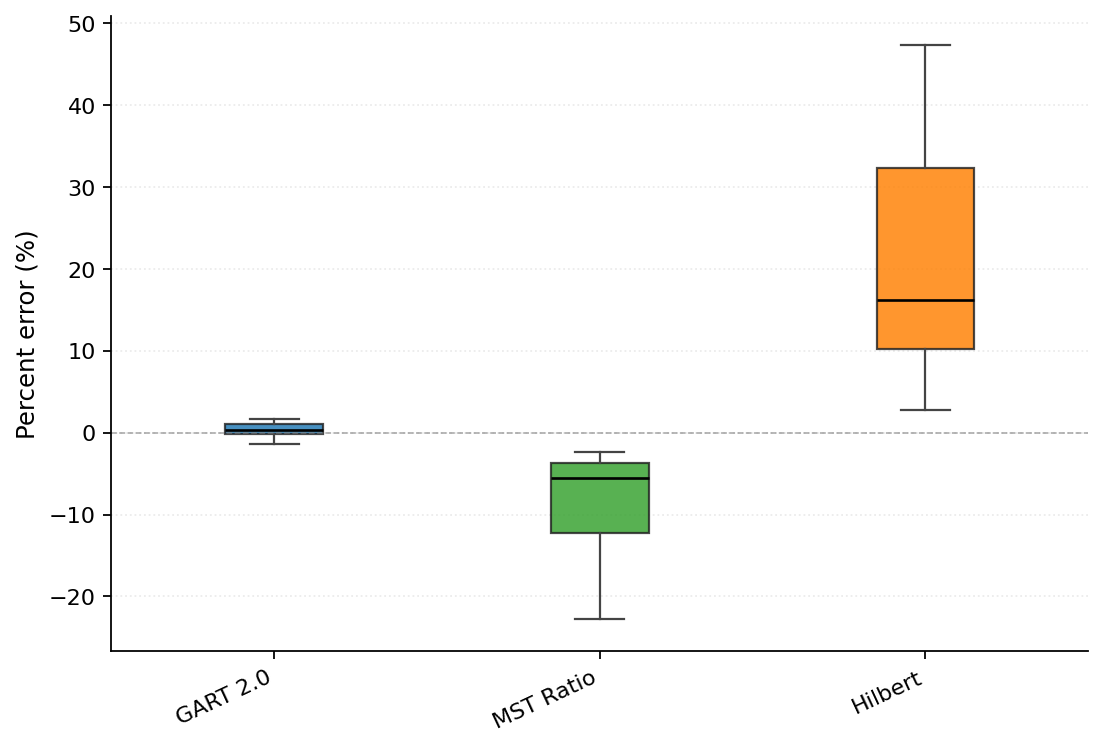
\includegraphics[width=0.75\textwidth]{boxplot_nd_errors.png}
\caption{Percent-error distribution per model on the multi-dimensional (ND) benchmark (16{,}920 instances).}
\label{fig:boxplot_nd}
\end{figure}

GART 2.0 reaches 0.88\% MAPE and 1.28\% SDPE overall, against 8.54\% / 6.84\% for MST Ratio and 21.20\% / 14.38\% for Hilbert (Figure~\ref{fig:boxplot_nd}). Precision tightens monotonically as $n$ grows (SDPE drops from 1.98\% at $n \le 10$ to 0.55\% at $n \in [501, 1000]$) and as $d$ grows (2.97\% at $d = 2$ down to 0.61\% at $d \in [30, 50]$), consistent with the theoretical convergence $\alpha \to 1$ in high dimensions \citep{percus1996finite}. The $d = 100$ bucket sits outside the training grid (which caps at $d = 50$) and therefore serves as a transfer test: the feature set must remain predictive at a dimension never seen during training. We acknowledge this is extrapolation in the favorable direction---$\alpha$ concentrates as $d$ grows, so the target variance shrinks with dimension; this is therefore not evidence of generalization. SDPE rises modestly from 0.61\% at $d \in [30, 50]$ to 0.65\% at $d = 100$, while MAPE moves from 0.38\% to 1.04\%. The two moves together describe a distribution-shift bias rather than a variance blow-up: the error distribution stays tight (SDPE tracks the shrinking target variance) but its center shifts slightly under genuine extrapolation, which is the benign failure mode for a precision-first estimator. MST Ratio (Table~\ref{tab:benchmark_models}) has nearly-flat SDPE because its fixed constant does not adapt to instance structure. Hilbert degrades with $n$ because space-filling locality breaks on non-uniform distributions. The favorable-direction extrapolation caveat noted above applies to every $d = 100$ row reported in this section.

\subsubsection{2D diverse benchmark} \label{subsec:results_2d}

The 2D diverse benchmark pushes every estimator against five distribution classes that probe distinct failure modes of classical geometry-based estimators. Across the 2{,}580 instances GART 2.0 holds SDPE under 6.3\% in every size bucket and under 3.3\% for instances with $n \ge 500$, with SDPE roughly half that of the MST-ratio baseline on the overall aggregate. Figure~\ref{fig:boxplot_2d} shows the per-model error distribution, and Table~\ref{tab:2d_by_size} dis-aggregates the results by instance size.

% tab:2d_by_size moved to Appendix~\ref{app:detail_2d}

\begin{figure}[!ht]
\centering
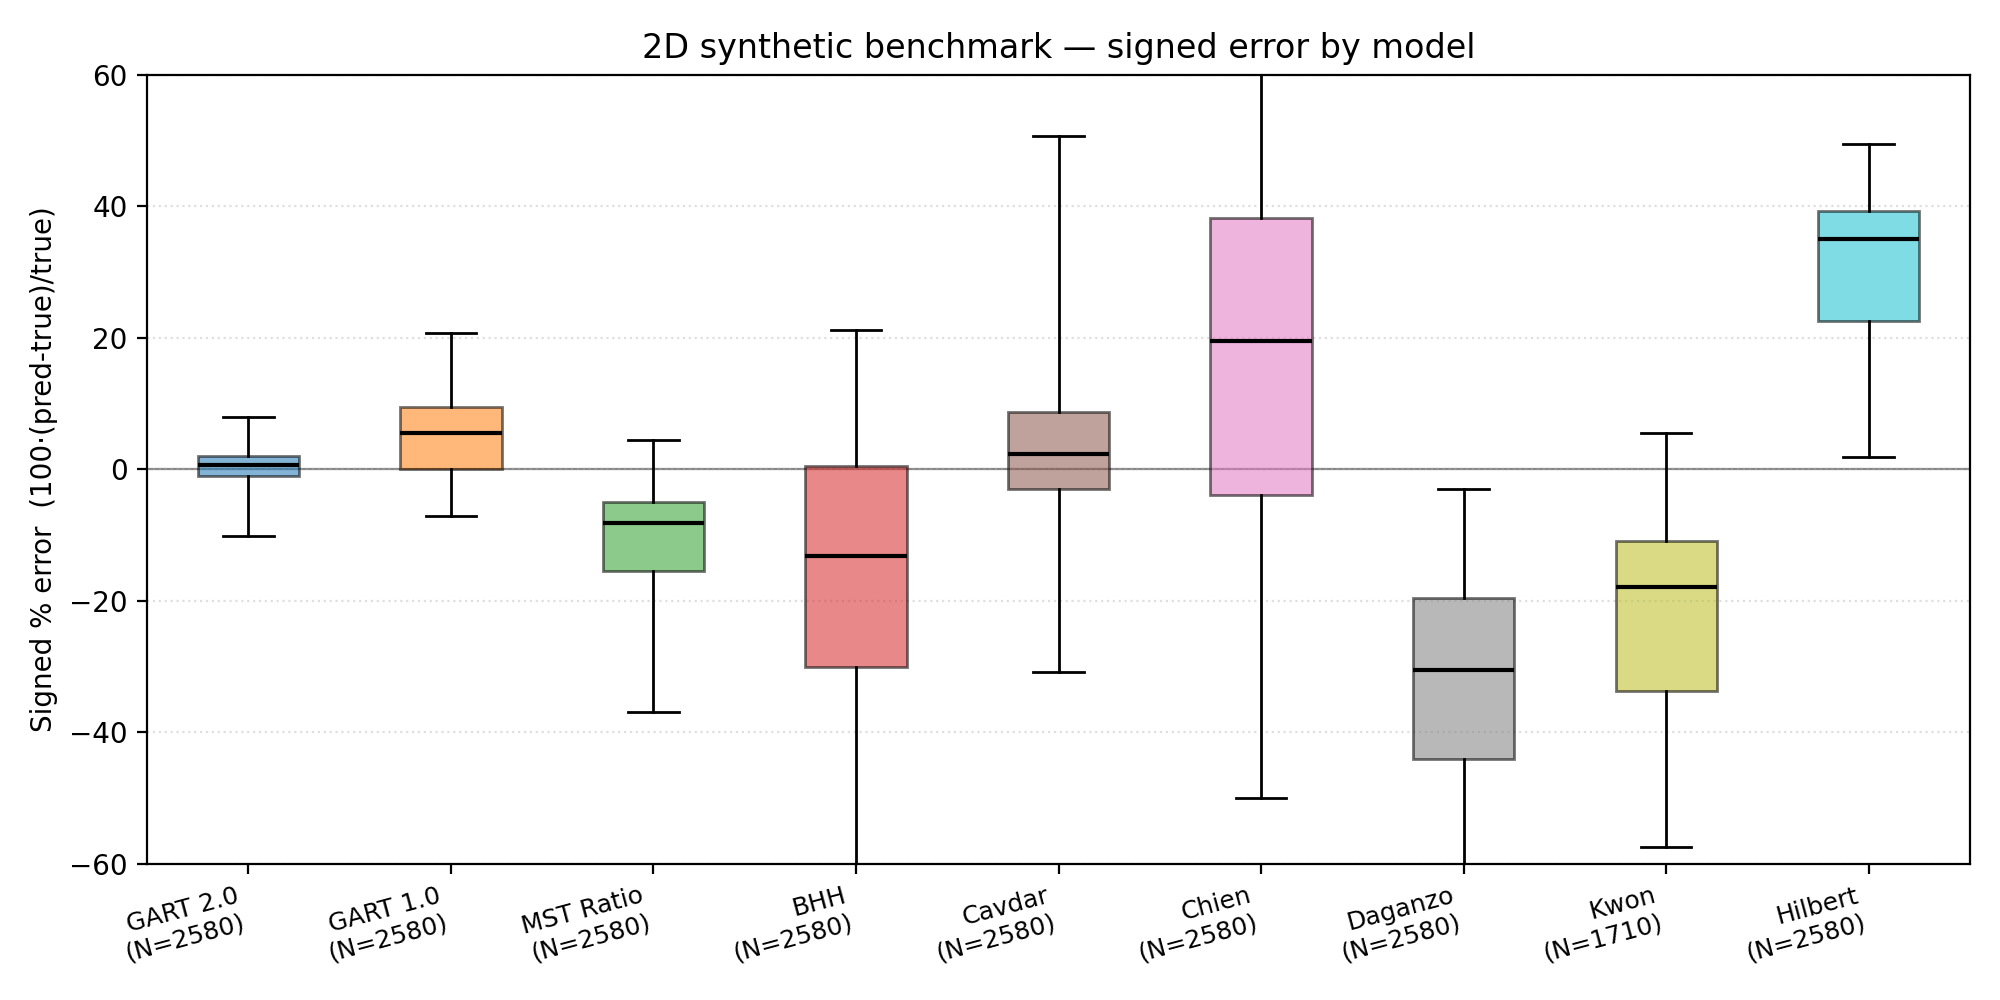
\includegraphics[width=0.75\textwidth]{boxplot_2d_errors.png}
\caption{Percent-error distribution per model on the 2D diverse benchmark (2{,}580 instances).}
\label{fig:boxplot_2d}
\end{figure}

GART 2.0 leads at 3.33\% MAPE / 5.19\% SDPE overall, with GART 1.0 \citep{gart2025} second among ML estimators at 7.35\% / 7.95\% --- the relative improvement over the predecessor model is most pronounced at $n \ge 200$, where GART 2.0's MST-centric features generalize to larger instances that GART 1.0's hull-based features cannot track. Among classical baselines, MST Ratio is strongest at 12.45\% / 11.06\%. The \c{C}avdar--Sokol estimator's MAPE drops by roughly an order of magnitude, from $\sim$160\% in earlier public adaptations of the formula to 16.13\% here, with SDPE tightening in parallel from $>200$\% to 32.19\%; the remaining spread still exceeds Kwon and Daganzo on this benchmark. The gain is traceable to the implementation corrections discussed in Appendix~\ref{app:bench_details} (rotation into the minimum-area bounding rectangle before evaluating per-axis statistics; the midpoint-axis distance in $\bar{c}_k$ rather than the centroid distance; the convex-hull area as $A$, following Section~5 of \citet{cavdar2015distribution}). BHH, Chien, and Daganzo all exceed 25\% SDPE because their enclosure-based formulas amplify variance on the Biased and Line Noise classes, where bounding-box and hull volumes diverge. Hilbert has intermediate MAPE (31\%) but lower SDPE (14\%): its errors are large but consistent --- a systematic space-filling bias. Kwon (1995) is structurally invalid above $n \approx 750$ (its linear $-0.0011\,n$ term forces the estimate negative) and is reported only where applicable.

\subsubsection{TSPLIB95 EUC\_2D benchmark} \label{subsec:results_tsplib}

Table~\ref{tab:tsplib_by_size} reports per-bucket results across all 78 EUC\_2D instances, with $n$ spanning 51 (\texttt{eil51}) to 18{,}512 (\texttt{d18512}). Bucket boundaries (23/16/39 instances) separate small, medium, and large real-world instances; the final $n>400$ bucket aggregates the asymptotic regime where classical MST-ratio calibration approaches its limit.

% tab:tsplib_by_size moved to Appendix~\ref{app:detail_tsplib}


\begin{figure}[!ht]
\centering
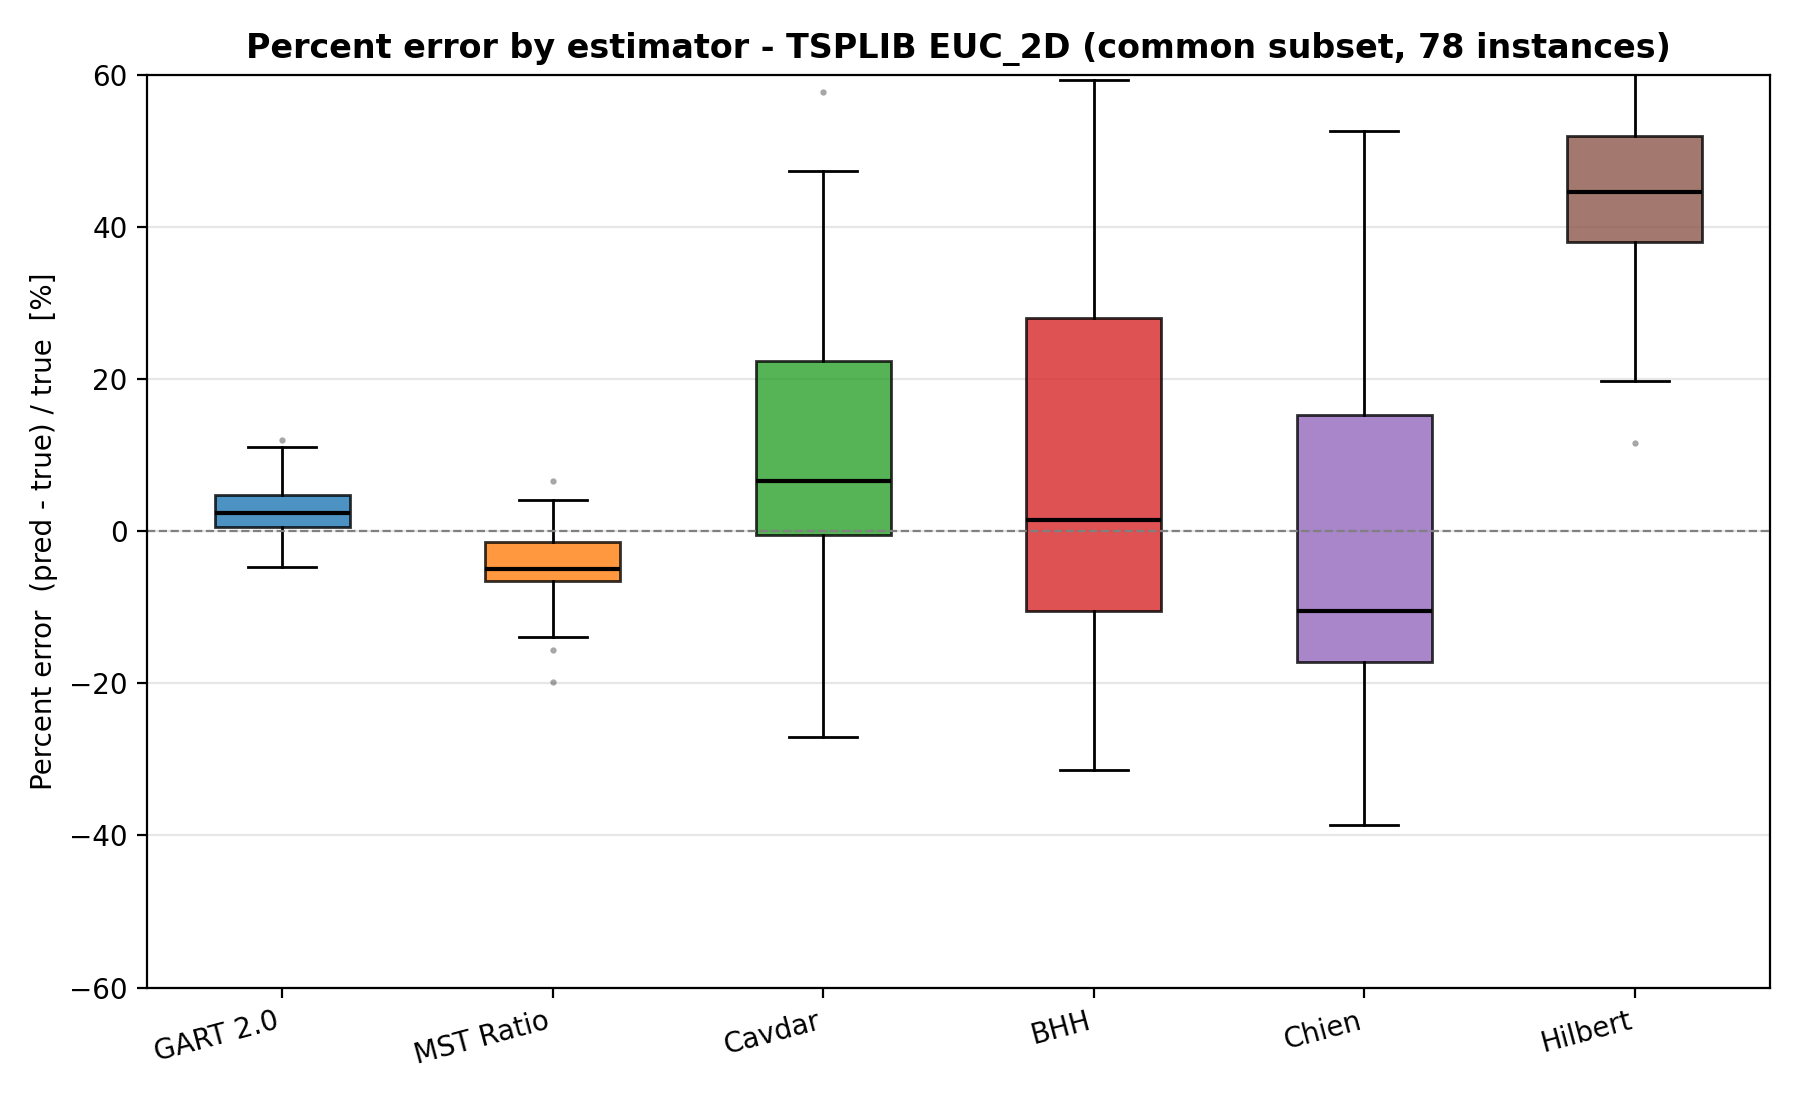
\includegraphics[width=0.75\textwidth]{boxplot_tsplib_errors.png}
\caption{Percent-error distribution per model on the TSPLIB95 EUC\_2D subset (78 instances).}
\label{fig:boxplot_tsplib}
\end{figure}

Real-world transfer is summarized in Figure~\ref{fig:boxplot_tsplib} and Table~\ref{tab:tsplib_by_size}: GART 2.0 retains the tightest SDPE in every bucket, though the margin collapses to 0.43 percentage points (3.42\% vs.\ 3.85\%) in the $n > 400$ bucket where MST Ratio's fixed constant matches the asymptotic $\alpha$ concentration and the two bootstrap intervals overlap. Overall GART 2.0 leads at SDPE 3.42\% / MAPE 3.27\% versus SDPE 4.54\% / MAPE 5.22\% for MST Ratio, the only classical baseline that stays competitive. GART 1.0 \citep{gart2025}, the prior 2D estimator, places second among ML models at SDPE 7.44\% / MAPE 8.46\%; its convex-hull-dependent features degrade on the largest instances, where GART 2.0's MST-centric redesign holds steady. Classical baselines BHH, \c{C}avdar--Sokol, Chien, and Daganzo degrade past $n = 400$ as real-world instances deviate from the uniform-density assumptions their derivations require. The largest instance in this subset, \texttt{d18512} ($n = 18{,}512$), is more than $18\times$ larger than any training instance and is predicted in under half a second. All 78 EUC\_2D instances run end-to-end for every model in this table with the total-time median for that instance across all models still well under a second.

\subsection{Discussion}

So far we have judged GART 2.0 on pointwise accuracy---how close each predicted tour cost is to the true optimum. Many of the downstream uses motivated in Section~\ref{sec:intro}, however, never consume a single cost value in isolation: they compare instances and act on the comparison, asking which candidate node set is cheaper or which route split to keep. For these uses the estimator must \emph{order} instances the way the true optima would, even when its absolute numbers are slightly off. We therefore close the benchmarking section by measuring this order agreement directly, with two standard rank correlations between predicted and true tour cost: Spearman's $\rho$, the correlation of the cost \emph{ranks}, and Kendall's $\tau$, the fraction of instance pairs the estimator orders concordantly with the truth. Both equal $1$ for a perfectly order-preserving estimator and $0$ for one unrelated to the truth.

Rank correlations on the same predictions used above confirm strong agreement: GART 2.0 reaches Spearman $\rho = 0.9993$ / Kendall $\tau = 0.981$ on the 2D benchmark, $\rho = 1.0000$ / $\tau = 0.998$ on the multi-dimensional set, and $\rho = 0.9991$ / $\tau = 0.985$ on TSPLIB EUC\_2D, outranking MST Ratio, GART 1.0, and Hilbert on both metrics in every case. The precision-first design is therefore also rank-preserving, exactly the property called for in Section~\ref{sec:intro} of an oracle intended for downstream optimization pipelines.

Global rank correlation near unity is compatible with local pairwise inversions in the dense part of the cost distribution, so we additionally report $\varepsilon$-close pairwise ranking accuracy---the fraction of instance pairs $(A, B)$ with $|L_A - L_B|/\max(L_A, L_B) < \varepsilon$ for which the estimator ranks $A, B$ in the same order as the true optima. At $\varepsilon = 5\%$ GART 2.0 reaches 70.9\% on TSPLIB EUC\_2D (55 qualifying pairs after excluding instances with ground-truth $\alpha > 2.5$ as degenerate outliers), 72.8\% on the 2D synthetic suite ($4.5 \times 10^{4}$ pairs), and 89.9\% on the multi-dimensional set ($2.3 \times 10^{4}$ pairs), versus 61.8\%, 71.0\%, and 71.7\% respectively for the fixed-MST-ratio baseline. At $\varepsilon = 10\%$ these rise to 78.3\%/82.0\%/94.7\%, again dominating the baseline in every slice. This pairwise-local metric is the signal a downstream planner sees when it must choose between two similar-cost candidates, and it is the one on which a global correlation near unity gives the least information; GART 2.0 leads the baseline on it uniformly, which we consider the operational content of the monotone-oracle framing.

This rank agreement is consistent with a classical asymptotic result that also explains when the fixed MST-ratio baseline catches up. For i.i.d.\ points of bounded density $f$ in $\mathbb{R}^d$, \citet{bhh1959} prove that $n^{-(d-1)/d} L_{\text{TSP}}(n) \to \beta(d) \int f^{(d-1)/d}$ almost surely, and \citet{steele1988growth} proves the analogous limit for the MST with its own constant $c(1,d)$ (the Steele theorem states $c(p, d)$ with edge-weight exponent $p=1$ corresponding to the MST, distinct from the MST-ratio $\alpha$ used elsewhere); dividing the two gives $L_{\text{TSP}}(n)/L_{\text{MST}}(n) \to \beta(d)/c(1,d)$ almost surely. In the $d = 100$ bucket MST Ratio already sits at 6.55\% MAPE against GART 2.0's 1.04\%, and in the largest TSPLIB bucket ($n > 400$) MST Ratio (3.92\%) matches GART 2.0 (3.75\%) on MAPE with essentially overlapping SDPE bootstrap intervals --- exactly the asymptotic regime in which the Beardwood--Steele ratio ceases to vary meaningfully with instance topology. GART 2.0's advantage is concentrated in the mid-density regime where finite-$n$ deviations from the asymptote dominate, which is also where practical logistics instances live.

The $n > 400$ TSPLIB bucket also exhibits $R^2_\alpha = -0.549$, which deserves direct acknowledgment rather than a footnote. The coefficient of determination is computed identically in both forms we audit---\texttt{sklearn.metrics.r2\_score} and the manual expression $1 - \text{SS}_{\text{res}}/\text{SS}_{\text{tot}}$---and the two agree to six decimal places, so the sign is not a bug. A negative value is legitimate under the sklearn convention whenever the estimator does worse than the per-bucket mean on $\alpha$, and three ingredients conspire to push $R^2_\alpha$ below zero on this slice: (i) real-world EUC\_2D $\alpha$ concentrates very tightly at large $n$, $\alpha \in [1.01, 1.20]$ with $\sigma(\alpha) \approx 0.044$, so the denominator $\text{SS}_{\text{tot}}$ is small; (ii) the model is pulled toward the synthetic-training prior whose mean $\alpha$ at matched $n$ is higher, producing a persistent upward offset; and (iii) the offset is monotone in $n$---mean $(\hat\alpha - \alpha)$ grows from $+0.006$ at $n \le 100$ to $+0.039$ at $n > 400$, with the fraction of over-predictions rising from 75\% to 87\% over the same range. The behavior is therefore a systematic distribution-shift bias between synthetic training and real-world TSPLIB geometry, not a variance problem: the SDPE column, which measures the tightness of the error distribution, remains the tightest in the table in every bucket including $n > 400$, because a consistent offset distorts $\alpha$ estimates far less than it distorts the absolute-ratio target $R^2_\alpha$. Cost-level accuracy ($R^2 = 1.000$, MAPE 3.75\%) is unaffected because $L_{\text{MST}}$ dominates $L_{\text{TSP}}$ at large $n$ and the multiplicative bias in $\alpha$ becomes a small additive tilt on tour cost. A future revision could correct the offset with a per-$n$ calibration layer; we note the limitation explicitly here rather than hide it in the table.

The classical geometric estimators --- BHH, \c{C}avdar--Sokol, Chien, Daganzo --- are absent from the ND results by construction: they require either the convex hull area or the bounding-box volume, and hull computation scales as $O(n^{\lfloor d/2 \rfloor})$ \citep{orourke1998} while the hull-to-box volume ratio shrinks exponentially with $d$ \citep{carlsson2024upper}.

The wall-time breakdown reflects the same MST-centric design. On the TSPLIB log --- the only timing log that cleanly separates preparation from inference --- GART 2.0 spends 84.8\% of its wall time on feature extraction and MST construction and 14.1\% on LightGBM inference, while classical baselines spend $\ge 99\%$ on feature and MST preparation. The overhead GART 2.0 introduces relative to any MST-based baseline is therefore the feature pipeline itself, not the tree ensemble; that pipeline cost is sunk as soon as the MST must be built. The remaining weak points are grid lattices and near-linear manifolds (Line Noise) where MST topology becomes structurally degenerate; both configurations are rare in real-world logistics but informative for mapping the model's boundary.

\section{Application: Non-Euclidean Estimation via MDS Embedding} \label{sec:application}

The preceding benchmarks evaluate GART 2.0 on Euclidean point clouds, where the MST is built directly from coordinates. Many real-world instances, however, provide no coordinates at all, or use a non-Euclidean metric that the coordinate-based feature pipeline cannot consume directly. This section extends the estimator to those cases with a multidimensional-scaling pre-step that produces a Euclidean embedding the same trained booster can read, and evaluates it on the non-EUC\_2D subset of TSPLIB95, where no classical 2D estimator is even defined.

TSPLIB95 contains 33 instances that are not native EUC\_2D: 4 CEIL\_2D (Euclidean with ceiling-rounded distances), 2 ATT (pseudo-Euclidean), 10 GEO (great-circle geographic), and 17 EXPLICIT (distance-matrix only). Classical estimators cannot process these: BHH and \c{C}avdar--Sokol require 2D coordinates, Chien requires convex hull area, and Hilbert requires a Euclidean embedding. Among our benchmarked baselines, GART 2.0 is the only one applicable to these cases. Timings are reported as an exploration of capability, not a comparison. We exclude the EXPLICIT outlier \texttt{brg180} from every aggregate because its distance matrix has 85{,}368 triangle-inequality violations: GART 2.0 (like any MST-based estimator) assumes symmetric metric distances, so non-metric instances are out of scope for this model. Excluding \texttt{brg180} leaves 32 metric instances (16 EXPLICIT) for evaluation.

\subsection{MDS preprocessing}

The following procedure converts any TSPLIB distance matrix into a Euclidean coordinate set that the GART 2.0 feature pipeline can consume unchanged. For each non-Euclidean TSPLIB instance we obtain a Euclidean coordinate representation by classical (metric) multidimensional scaling \citep{torgerson1952mds,gower1966some,borg2005mds,cox2000mds}: we double-center the squared distance matrix $D^{(2)}$ and take the leading eigenvectors of the resulting Gram matrix \citep{gower1966some}. We use the SciPy eigendecomposition routine \citep{scipy2020} and retain the smallest embedding dimension $k$ that preserves $\ge 99.9\%$ of the positive eigenvalue mass (capped at $k = 100$). A non-Euclidean instance has no native coordinate dimension $d$, so we write $k$ rather than $d$ for the number of dimensions the embedding produces; this $k$ takes the role that $d$ plays for Euclidean inputs. Geometric features are computed on the $k$-dimensional MDS embedding while MST features are computed from the original distance matrix $D$ so no metric information is lost, and the selected $k$ is passed to the model as the \texttt{dimension} feature. Full derivation and the per-instance $k$ distribution are given in Appendix~\ref{app:mds}.

\subsection{Results on non-Euclidean TSPLIB95}

\begin{table}[!ht]
\centering
\caption{GART 2.0 on non-Euclidean TSPLIB95 (32 instances, \texttt{brg180} excluded).}
\label{tab:tsplib_nonEuc}
\resizebox{\textwidth}{!}{%
\footnotesize
\begin{tabular}{@{}l r l r r r r c@{}}
\toprule
Distance type & Count & SDPE (\%) [95\% CI] & MAPE (\%) & $|$Median$|$ (\%) & $r_\alpha$ & Time (ms) & Embed.\ $k$ (avg [range]) \\
\midrule
ATT             & 2  & 0.48 \scriptsize[---,\,---]         & 4.65 & 4.65 & ---       & 23.4 & 53 [6,100] \\
CEIL\_2D        & 4  & 6.12 \scriptsize[0.74,\,7.49]       & 6.49 & 6.15 & $+0.656$  & 211  & 2 [2,2]    \\
GEO             & 10 & 2.18 \scriptsize[0.68,\,2.97]       & 3.92 & 4.57 & $+0.982$  & 9.3  & 16 [2,61]  \\
EXPLICIT-metric & 16 & 5.90 \scriptsize[3.78,\,7.43]       & 6.22 & 5.46 & $+0.868$  & 7.6  & 37 [8,100] \\
\midrule
\textbf{TOTAL}  & \textbf{32} & \textbf{5.56} \scriptsize[\textbf{3.86},\,\textbf{6.99}] & \textbf{5.43} & \textbf{4.99} & \textbf{+0.868} & \textbf{9.2} & --- \\
\bottomrule
\end{tabular}%
}
\end{table}

The embedded dimension $k$ is chosen adaptively per instance by the MDS variance-retention rule, and $r_\alpha$ is undefined for the ATT row because only two instances are available. No \textsc{Concorde} or \textsc{LKH-3} solver time is reported: neither solver is natively applicable to non-Euclidean distance types without format-specific translation, which falls outside the scope of this experiment. As reported in Table~\ref{tab:tsplib_nonEuc}, GART 2.0 generalizes across all four distance types at an aggregate SDPE of 5.56\% and MAPE of 5.43\% over the 32 instances, with the per-type MAPE spanning 3.92--6.49\%. GEO instances achieve the lowest error (MAPE 3.92\%) because great-circle distances admit a low-stress Euclidean embedding at typical geographic scales. EXPLICIT-metric instances reach 6.22\% because their matrices may mildly violate the triangle inequality, inflating MDS stress. The CEIL\_2D row's comparatively high 211~ms time should not be read as a typical per-instance cost: that group contains only four instances, two of them larger than $n = 10{,}000$, so its median is dominated by those two large cases rather than representative of the distance type.

\section{Conclusion}\label{sec:conclusion}

We presented GART 2.0, a TSP tour-length estimator that predicts the MST-to-TSP scaling factor $\alpha$ using 30 dimension-agnostic features combining MST topology with lightweight coordinate-range descriptors. Across 2{,}580 synthetic 2D instances, 16{,}920 multi-dimensional test instances spanning $d = 2$ to $d = 100$, and 110 metric TSPLIB95 instances (78 EUC\_2D and 32 non-Euclidean via MDS), MST-topology features recover the per-instance scaling factor with high precision and monotonicity across dimensions and distribution types, without any enclosure geometry. The primary contribution is a monotone, precision-first estimator: its SDPE is materially tighter than the MST-ratio baseline and its error ordering tracks the true cost ordering, so it can serve as a rank-preserving oracle inside a larger optimization pipeline. It outperforms the MST-ratio baseline on every benchmark, including the 78 EUC\_2D TSPLIB95 instances whose largest $n = 18{,}512$ is more than $18\times$ the training cap; the Delaunay-accelerated feature pipeline yields sub-500~ms prediction at $n = 1{,}000$. Because a single MDS-hybrid pipeline lets GART 2.0 handle every metric TSPLIB95 distance type---EUC\_2D, CEIL\_2D, ATT, GEO, and EXPLICIT---it applies to a broader range of real-world instances than the classical estimators we benchmark, which are restricted to 2D Euclidean inputs.

Three limitations point at concrete next steps. The $\alpha$ regressor is not yet tight: the coefficient of determination on $\alpha$ and related diagnostics in the benchmarking tables show that a non-trivial share of the target variance is still unexplained, and a more expressive regressor such as a deeper LightGBM, a small neural head on the current features, or a probabilistic model targeting the conditional distribution of $\alpha$ should reduce SDPE further without new feature engineering. Feature extraction time still scales with $d$ even though feature definitions do not, because pairwise distances, centroid statistics, and MST construction all scale with $d$; a principled dimension-reduction front-end such as a learned embedding or random projection would make dimension-independence hold in cost as well as in definition. At large $n$ under near-uniform spatial density, the true $\alpha$ concentrates tightly around its asymptotic BHH value and a constant-$\alpha$ estimator is already comparable to GART 2.0 at lower cost; GART 2.0's precision advantage is strongest at lower $n$ and under distributions that deviate from uniform, so a dispatch layer that runs the MST-ratio baseline in the easy regime and defers to GART 2.0 otherwise is a natural follow-on. A separate next step is to embed the estimator inside a larger optimization loop, such as a Vehicle Routing Problem sub-tour estimator \citep{frontiers2021} or a bounding function in branch-and-bound, to measure whether the precision advantage translates into faster, more reliable end-to-end decisions.

%Bibliography
\clearpage % flush pending todonotes/floats before appendix (prevents "Float(s) lost")
\bibliographystyle{plainnat}
\bibliography{references}

\clearpage
\appendix

\section{Code and Data Availability} \label{app:code}

Our implementation, trained model weights, and benchmark scripts are available at \url{https://github.com/sfeldmanMIG25/Area-and-Distribution-Free-Estimator-for-TSP}. Synthetic instances can be regenerated using the provided scripts with fixed random seeds.

The GART 2.0 pipeline is implemented in Python using SciPy \citep{scipy2020} for Delaunay triangulation \citep{delaunay1934} and MST construction (via \texttt{scipy.sparse.csgraph.minimum\_spanning\_tree}), Numba \citep{numba2015} for JIT-compiled centroid distance computation, and scikit-learn \citep{sklearn2011} for classical MDS embedding of non-Euclidean distance matrices. For instances without Euclidean coordinates (e.g., TSPLIB GEO and EXPLICIT types), MDS projects the distance matrix into Euclidean coordinates for geometric feature extraction while MST features are computed from the original distances; details are given in Appendix~\ref{app:mds} and evaluated in Section~\ref{sec:application}. The LightGBM model \citep{ke2017lightgbm} is trained and served via the Python API. All benchmarks were run on a single machine (Intel i7 13th Gen, 64\,GB RAM, Windows 11). Concorde version 03.12.19 and LKH-3 version 3.0.13 were used for ground-truth computation.

\section{Training Data Generation Details} \label{app:training}

The training dataset was constructed by generating synthetic TSP instances across four distribution classes, with dimensions independently assigned per axis:

The uniform class draws coordinates from $\mathcal{U}(0, G)$ where $G$ is the grid size. The normal class draws from $\mathcal{N}(G/2, G/6)$ truncated to $[0, G]$. The clustered class places $k \in [3, 15]$ cluster centers uniformly and draws points from $\mathcal{N}(\mu_k, \sigma_k)$ around each center. The correlated class uses autoregressive structure across dimensions, $x_{d+1} = \rho \cdot x_d + \epsilon$, producing axis-aligned anisotropy.

Each instance's dimensions are independently assigned a distribution class, producing anisotropic configurations where topology varies by axis. Node counts span $n \in [5, 1{,}000]$ with training-visible dimensions $d \in \{2, 3, 4, 5, 6, 7, 8, 9, 10, 15, 20, 25, 30, 35, 40, 45, 50\}$ (17 dimension values), plus a held-out extrapolation bucket at $d = 100$ ($5{,}904$ instances, all placed in the test split). Ground-truth solutions were computed by running both Concorde and LKH-3, retaining the shorter result.

The $106{,}272$ solved instances are partitioned into training ($69{,}768$, $65.6\%$), validation ($19{,}584$, $18.4\%$), and test ($16{,}920$, $15.9\%$) using a stratified sample on $(d, n, \text{grid size})$. The stratification rule ranks instances within each stratum by a seeded uniform and assigns roughly the first 16\% to test, the next 18\% to validation, and the remainder to training; $d = 100$ instances bypass this rule and are locked to the test partition (see \texttt{feature\_creator\_v3.create\_stratified\_split}). Table~\ref{tab:training_grid} lists the per-$(d, n)$ training-instance count; grid size $G \in \{100, 1{,}000, 10{,}000\}$ is sampled uniformly within each cell.

\subsection{Multi-dimensional benchmark grid} \label{app:nd_grid_counts}

For reference, the full $(d, n)$ count grid of the 16{,}920-instance ND benchmark:

\begin{table}[H]
\centering
\caption{Multi-dimensional synthetic benchmark grid: instance count per $(d, n)$ bucket (16{,}920 instances total).}
\label{tab:nd_grid_counts}
\resizebox{\textwidth}{!}{%
\footnotesize
\begin{tabular}{@{}l rrrrrr|r@{}}
\toprule
$d$ \textbackslash\ $n$ & $[5,10]$ & $[11,50]$ & $[51,100]$ & $[101,200]$ & $[201,500]$ & $[501,1000]$ & Total \\
\midrule
$d=2$ & 162 & 108 & 135 & 27 & 81 & 135 & \textbf{648} \\
$d=3$--$5$ & 486 & 324 & 405 & 81 & 243 & 405 & \textbf{1{,}944} \\
$d=6$--$10$ & 810 & 540 & 675 & 135 & 405 & 675 & \textbf{3{,}240} \\
$d=15$--$25$ & 486 & 324 & 405 & 81 & 243 & 405 & \textbf{1{,}944} \\
$d=30$--$50$ & 810 & 540 & 675 & 135 & 405 & 675 & \textbf{3{,}240} \\
$d=100$ & 1{,}476 & 984 & 1{,}230 & 246 & 738 & 1{,}230 & \textbf{5{,}904} \\
\midrule
\textbf{Total} & \textbf{4{,}230} & \textbf{2{,}820} & \textbf{3{,}525} & \textbf{705} & \textbf{2{,}115} & \textbf{3{,}525} & \textbf{16{,}920} \\
\bottomrule
\end{tabular}%
}
\end{table}

\begin{table}[H]
\centering
\caption{Training-set instance count per $(d, n)$ cell ($69{,}768$ total; grid size $G \in \{100,\,1{,}000,\,10{,}000\}$ sampled uniformly within each cell; four distribution classes per axis listed in \S\ref{app:training}).}
\label{tab:training_grid}
\resizebox{\textwidth}{!}{%
\footnotesize
\begin{tabular}{@{}l rrrrrr|r@{}}
\toprule
$d$ \textbackslash\ $n$ & $[5,10]$ & $[11,50]$ & $[51,100]$ & $[101,200]$ & $[201,500]$ & $[501,1000]$ & Total \\
\midrule
$d=2$ & 1{,}026 & 684 & 855 & 171 & 513 & 855 & \textbf{4{,}104} \\
$d=3$--$5$ & 3{,}078 & 2{,}052 & 2{,}565 & 513 & 1{,}539 & 2{,}565 & \textbf{12{,}312} \\
$d=6$--$10$ & 5{,}130 & 3{,}420 & 4{,}275 & 855 & 2{,}565 & 4{,}275 & \textbf{20{,}520} \\
$d=15$--$25$ & 3{,}078 & 2{,}052 & 2{,}565 & 513 & 1{,}539 & 2{,}565 & \textbf{12{,}312} \\
$d=30$--$50$ & 5{,}130 & 3{,}420 & 4{,}275 & 855 & 2{,}565 & 4{,}275 & \textbf{20{,}520} \\
\midrule
\textbf{Total} & \textbf{17{,}442} & \textbf{11{,}628} & \textbf{14{,}535} & \textbf{2{,}907} & \textbf{8{,}721} & \textbf{14{,}535} & \textbf{69{,}768} \\
\bottomrule
\end{tabular}%
}
\end{table}

\section{Detailed Feature Specifications} \label{app:features}

Tables~\ref{tab:edge_features} and~\ref{tab:topo_features} list the 22 MST-derived features used by GART 2.0, complementing the geometric features of Table~\ref{tab:geo_features} (\S\ref{subsec:features}). Listed complexities assume the MST has already been built; MST construction itself dominates the asymptotic cost and is analyzed in \S\ref{sec:methodology}.

\subsection{MST Edge Distribution Statistics} \label{app:features_edge}

The second category captures the local uniformity of the point set through the statistical moments of the MST edge weights. Unlike coordinate-based variance, edge weights are invariant to rotation and translation. High skewness or kurtosis in this distribution typically indicates a mixture of scales, such as dense clusters separated by voids, which significantly impacts the $\alpha$ ratio.

\begin{table}[H]
\centering
\caption{MST Edge Statistic Specifications}
\label{tab:edge_features}
\resizebox{\textwidth}{!}{%
\begin{tabular}{@{}lp{6.5cm}ll@{}}
\toprule
\textbf{Feature Name} & \textbf{Description \& Rationale} & \textbf{Complexity} & \textbf{Origin / Citation} \\ \midrule
\textbf{MST Edge Max} & Weight of the longest edge in the MST. & $O(n)$ & Standard \\
\textbf{MST Quantiles} & 10\%, 25\%, 50\%, 75\%, 90\% percentiles. Provides a non-parametric distribution profile. & $O(n \log n)$ & \textbf{Proposed}; via MST \citep{prim1957} \\
\textbf{MST Total Length} & Sum of all edge weights. The primary scaling factor; $L_{\text{TSP}} \ge L_{\text{MST}}$. & $O(n^2)$ & \citet{prim1957} \\
\textbf{MST Edge Mean} & Average edge length in the MST. & $O(n)$ & \citet{smithmiles2010} \\
\textbf{MST Edge Std} & Standard deviation of edge lengths in the MST. & $O(n)$ & \citet{smithmiles2010} \\
\textbf{MST Edge Skewness} & Asymmetry of edge distribution. High positive skew implies many short edges and few long bridges. & $O(n)$ & \citet{smithmiles2010} \\
\textbf{MST Edge Kurtosis} & Tailedness of distribution. Indicates the presence of extreme outliers. & $O(n)$ & \citet{smithmiles2010} \\  \bottomrule
\end{tabular}%
}
\end{table}

\subsection{Topological Structure and Clustering Proxies} \label{app:features_topo}

The final category contains features designed to detect higher-order structures—such as clusters, filaments, and hubs—without performing expensive clustering algorithms. We introduce specific ratios (Dominance, Gap, Normalized Diameter) that serve as $O(n)$ proxies for these complex geometric properties. For instance, the "Leaf Ratio" effectively distinguishes between low-dimensional linear manifolds (low leaf count) and high-dimensional isotropic noise (high leaf count).

\begin{table}[H]
\centering
\caption{Topological and Clustering Feature Specifications}
\label{tab:topo_features}
\resizebox{\textwidth}{!}{%
\begin{tabular}{@{}lp{6.5cm}ll@{}}
\toprule
\textbf{Feature Name} & \textbf{Description \& Rationale} & \textbf{Complexity} & \textbf{Origin / Citation} \\ \midrule
\textbf{MST Dominance Ratio} & Sum of largest $\sqrt{n}$ edges / Total Length. Captures weight of inter-cluster bridges. & $O(n)$ & \textbf{Proposed}; via MST \citep{prim1957} \\
\textbf{MST Gap Ratio} & Max edge / Median edge. Measures magnitude of sparsity jumps. & $O(1)$ & \textbf{Proposed}; via MST \citep{prim1957} \\
\textbf{MST Leaf Ratio} & Fraction of nodes with degree $k=1$. Topology proxy for dimensionality. & $O(n)$ & \citet{smithmiles2010} \\
\textbf{MST Degree (Mean, Std)} & Branching factor statistics. & $O(n)$ & \citet{smithmiles2010} \\
\textbf{MST Degree Max} & Maximum node degree. Identifies "hub" nodes common in High-D spaces. & $O(n)$ & \citet{smithmiles2010} \\
\textbf{MST Diameter} & Sum of edge weights on the longest path between any two leaves, computed via double-BFS. & $O(n)$ & Graph Theory \\
\textbf{Normalized Diameter} & Diameter / Total Length. Scale-invariant shape proxy ($=1.0$ for path-manifolds exactly). & $O(1)$ & \textbf{Proposed}; via double-BFS \\
\textbf{Large Edge Count} & Count of edges $> \mu + \sigma$. Secondary cluster indicator. & $O(n)$ & \textbf{Proposed}; via MST \citep{prim1957} \\ \bottomrule
\end{tabular}%
}
\end{table}

\section{Feature Importance: SHAP Values} \label{app:shap}

To validate the 30-feature set, we report the SHAP values \citep{lundberg2017shap} on the held-out test split using the saved booster (see \texttt{shap\_analyzer\_v3.py}). Table~\ref{tab:shap_top} ranks all 30 features by mean absolute SHAP contribution. Three observations motivate the final feature set.

First, the MST dominance ratio alone carries 26.4\% of the model's decision mass, and six of the top ten features are MST-derived (dominance ratio, degree mean, diameter, diameter-normalized, gap ratio, large-edge count). This is consistent with the BHH intuition that tour length scales with tree-like spanning structure; it also justifies the decision to feature-engineer from the MST rather than from raw coordinates. Second, dimension and size are first-class inputs. $n$ and $d$ together contribute 22.2\% of the decision mass, which is how the model adapts to varying problem scale without being given a distribution label. Finally, lightweight spread statistics add coverage. Centroid-distance dispersion (4.8\% share on \texttt{centroid\_dist\_std} alone, 9.9\% summed across the four centroid-distance descriptors) and bounding hypervolume ($\sim$4.6\% summed across the log and linear forms) contribute meaningfully once evaluated in the canonical principal-axis frame (\S\ref{subsec:features}), which is what allows the rotation-sensitive block to carry signal without leaking orientation noise and without requiring a convex-hull computation, keeping the feature set applicable at arbitrary $d$.

Additional testing showed that introducing further features found in literature such as a Greedy Nearest Neighbor Tour led to overfitting with the model learning the underlying distributions from the training data rather than generalizing. SHAP analysis was used to iteratively reduce the features chosen to the 30 features discussed in \ref{subsec:features}.

\begin{table}[H]
\centering
\caption{All 30 features of GART 2.0 ranked by mean $|$SHAP$|$ (held-out test split, $N=2{,}000$ sampled rows, seed 42, recomputed on the current trained booster). The bar shows the share of total SHAP mass.}
\label{tab:shap_top}
\setlength{\tabcolsep}{6pt}
\renewcommand{\arraystretch}{1.1}
\rowcolors{2}{gray!5}{white}
\begin{tabular}{@{}rlrrl@{}}
\toprule
\textbf{Rank} & \textbf{Feature} & \textbf{Mean $|$SHAP$|$} & \textbf{Share (\%)} & \textbf{} \\
\midrule
1  & \texttt{mst\_dominance\_ratio}      & 0.0388 & 26.43 & \textcolor{blue!70!black}{\rule{26.4mm}{4pt}} \\
2  & \texttt{dimension}                  & 0.0171 & 11.66 & \textcolor{blue!70!black}{\rule{11.7mm}{4pt}} \\
3  & \texttt{n\_customers}               & 0.0155 & 10.55 & \textcolor{blue!70!black}{\rule{10.6mm}{4pt}} \\
4  & \texttt{centroid\_dist\_std}        & 0.0071 &  4.81 & \textcolor{blue!70!black}{\rule{4.8mm}{4pt}} \\
5  & \texttt{mst\_degree\_mean}          & 0.0068 &  4.62 & \textcolor{blue!70!black}{\rule{4.6mm}{4pt}} \\
6  & \texttt{mst\_diameter}              & 0.0063 &  4.30 & \textcolor{blue!70!black}{\rule{4.3mm}{4pt}} \\
7  & \texttt{mst\_diameter\_normalized}  & 0.0061 &  4.18 & \textcolor{blue!70!black}{\rule{4.2mm}{4pt}} \\
8  & \texttt{mst\_gap\_ratio}            & 0.0050 &  3.39 & \textcolor{blue!70!black}{\rule{3.4mm}{4pt}} \\
9  & \texttt{large\_edge\_count}         & 0.0044 &  2.98 & \textcolor{blue!70!black}{\rule{3.0mm}{4pt}} \\
10 & \texttt{bounding\_hypervolume}      & 0.0040 &  2.70 & \textcolor{blue!70!black}{\rule{2.7mm}{4pt}} \\
11 & \texttt{mst\_leaf\_ratio}           & 0.0039 &  2.66 & \textcolor{blue!70!black}{\rule{2.7mm}{4pt}} \\
12 & \texttt{mst\_degree\_max}           & 0.0034 &  2.32 & \textcolor{blue!70!black}{\rule{2.3mm}{4pt}} \\
13 & \texttt{centroid\_dist\_mean}       & 0.0030 &  2.05 & \textcolor{blue!70!black}{\rule{2.1mm}{4pt}} \\
14 & \texttt{log\_bounding\_hypervolume} & 0.0027 &  1.85 & \textcolor{blue!70!black}{\rule{1.9mm}{4pt}} \\
15 & \texttt{centroid\_dist\_max}        & 0.0024 &  1.61 & \textcolor{blue!70!black}{\rule{1.6mm}{4pt}} \\
16 & \texttt{centroid\_dist\_iqr}        & 0.0022 &  1.51 & \textcolor{blue!70!black}{\rule{1.5mm}{4pt}} \\
17 & \texttt{mst\_edge\_max}             & 0.0020 &  1.35 & \textcolor{blue!70!black}{\rule{1.4mm}{4pt}} \\
18 & \texttt{mst\_edge\_q75}             & 0.0017 &  1.19 & \textcolor{blue!70!black}{\rule{1.2mm}{4pt}} \\
19 & \texttt{aspect\_ratio}              & 0.0017 &  1.13 & \textcolor{blue!70!black}{\rule{1.1mm}{4pt}} \\
20 & \texttt{mst\_degree\_std}           & 0.0016 &  1.11 & \textcolor{blue!70!black}{\rule{1.1mm}{4pt}} \\
21 & \texttt{log\_node\_density}         & 0.0015 &  1.01 & \textcolor{blue!70!black}{\rule{1.0mm}{4pt}} \\
22 & \texttt{mst\_edge\_q90}             & 0.0014 &  0.97 & \textcolor{blue!70!black}{\rule{0.97mm}{4pt}} \\
23 & \texttt{mst\_edge\_q25}             & 0.0014 &  0.93 & \textcolor{blue!70!black}{\rule{0.93mm}{4pt}} \\
24 & \texttt{mst\_edge\_mean}            & 0.0012 &  0.81 & \textcolor{blue!70!black}{\rule{0.81mm}{4pt}} \\
25 & \texttt{node\_density}              & 0.0011 &  0.76 & \textcolor{blue!70!black}{\rule{0.76mm}{4pt}} \\
26 & \texttt{mst\_edge\_skew}            & 0.0011 &  0.72 & \textcolor{blue!70!black}{\rule{0.72mm}{4pt}} \\
27 & \texttt{mst\_edge\_q10}             & 0.0010 &  0.70 & \textcolor{blue!70!black}{\rule{0.70mm}{4pt}} \\
28 & \texttt{mst\_edge\_q50}             & 0.0010 &  0.68 & \textcolor{blue!70!black}{\rule{0.68mm}{4pt}} \\
29 & \texttt{mst\_edge\_kurtosis}        & 0.0009 &  0.59 & \textcolor{blue!70!black}{\rule{0.59mm}{4pt}} \\
30 & \texttt{mst\_edge\_std}             & 0.0006 &  0.41 & \textcolor{blue!70!black}{\rule{0.41mm}{4pt}} \\
\bottomrule
\end{tabular}
\end{table}

\section{Benchmark-Model Implementation Notes} \label{app:bench_details}

This appendix records per-baseline implementation details that were removed from \S\ref{subsec:bench_models} for brevity.

\paragraph{BHH constant.} For $d=2$ we use the large-scale empirical estimate $\beta_2 = 0.7124 \pm 0.0002$ of \citet{johnson1996asymptotic} from Concorde-verified optima on uniform random point sets; an independent statistical-mechanics study \citep{percus1996finite} reports $\beta_2 = 0.7120 \pm 0.0002$ under toroidal boundary conditions. We retain $0.7124$ because our benchmark consumes uniform point sets under open (square) boundaries. \citet{cerf1997tsp} reports $\beta_3 = 0.6979 \pm 0.0002$ for the 3D case; we do not apply BHH for $d \ge 3$ because the hull-to-bounding-box volume ratio decays exponentially with dimension, making $V$ unstable as an estimator \citep{carlsson2024upper}.

\paragraph{\c{C}avdar--Sokol.} Regression coefficients are $\alpha_1 = 2.791$, $\alpha_2 = 0.2669$ as fitted in \citet{cavdar2015distribution}; $A$ is convex-hull area, $\sigma_k$ is the standard deviation of coordinates in dimension $k$, $\bar c_k$ is the average absolute distance from each node to the \emph{midpoint axis} of the bounding rectangle in dimension $k$ (i.e.\ to the line $x_k = (\max_k + \min_k)/2$, not to the coordinate mean), and $\sigma'_k$ is the standard deviation of those absolute distances. Because the original model was trained on axis-aligned rectangular graphs, we rotate coordinates into the minimum-area bounding rectangle using rotating calipers over the convex hull \citep{freeman1975determining} before computing dispersion. For $n < 1000$ we apply the small-$n$ correction $E/T = 0.9325\,e^{0.00005298\,n} - 0.2972\,e^{-0.01452\,n}$ from \citet[Eq.~4]{cavdar2015distribution}.

\paragraph{Kwon--Golden--Wasil.} $R$ is the mean centroid distance, a depot-free adaptation of Kwon's depot-to-region distance. The linear $-0.0011\,n$ term was calibrated for VRP customer counts in the tens-to-hundreds range; extrapolated to $n$ in the thousands it drives the prediction negative, which we clip to zero. To stabilize the formula across TSPLIB's wide coordinate-scale range, we rescale coordinates so the bounding-box diagonal is $1$, evaluate Kwon in that normalized space, and multiply the result by the original diagonal. Both behaviors are visible in Table~\ref{tab:tsplib_by_size}: Kwon tracks the data for $n \le 400$ and degenerates for $n \ge 1500$.

\paragraph{Daganzo vs.\ BHH.} Structurally Daganzo is BHH with a different constant: the $0.57$ coefficient is the CVRP calibration of \citet{daganzo1984a}, visibly looser than the BHH/uniform-square value $0.7124$. We include both because the literature reports them as distinct benchmarks.

\paragraph{Chien.} $A$ is convex-hull area, $n$ stops, $p$ routes; we set $k_1 = 0.98$, $k_2 = 0$, $p = 1$ for single-tour evaluation.

\paragraph{Hilbert curve.} The constructive heuristic of \citet{bartholdi1982heuristic} originally used a Sierpinski-style space-filling curve; the Hilbert variant we implement here is a later refinement in the same family. Points are sorted by their Hilbert index $h(x)$ and visited in that order.

\paragraph{MST Ratio constants.} For $d=2$ we use $\rho(2) = 1.075$ computed as $\beta_{\text{TSP}}(2)/\beta_{\text{MST}}(2) \approx 0.7124/0.663$ \citep{johnson1996asymptotic, cortinaborja2000mst}, consistent with the analytic lower bound of $0.6008$ on $\beta_{\text{MST}}(2)$ from \citet{avram1992mst}. For higher dimensions we use the empirical schedule $\rho(3) = 1.05$ and $\rho(d) = 1.0 + 0.075 \cdot (2/d)$ for $d \ge 4$. This schedule is not taken from prior work; we constructed it to interpolate monotonically between the calibrated $d=2$ value and the $d \to \infty$ limit of unity established by \citet{percus1996finite}, and treat it as a baseline to be compared against, not as a calibrated MST-to-TSP relationship for arbitrary $d$. These constants are calibrated for uniform distributions; the elevated SDPE observed for MST Ratio in Table~\ref{tab:nd_by_dim} reflects the inability of a fixed constant to adapt to topological variation in non-uniform test instances.

\section{Per-Dimension Detail for the Multi-Dimensional Benchmark} \label{app:nd_detail_dim}

Table~\ref{tab:nd_by_dim} reports the multi-dimensional benchmark broken down by dimension $d$.

\begin{table}[H]
\centering
\caption{ND benchmark by dimension; same 16{,}920 instances as Table~\ref{tab:nd_by_size}.}
\label{tab:nd_by_dim}
\resizebox{\textwidth}{!}{%
\footnotesize
\renewcommand{\arraystretch}{1.15}
\begin{tabular}{@{}l l rrrrrr@{}}
\toprule
Bucket & Model & SDPE (\%) [95\% CI] & MAPE (\%) & $|$Median$|$ (\%) & $R^2$ & $R^2_\alpha$ & Time (ms) \\
\midrule
\multirow{4}{*}{\makecell[l]{$d=2$\\ Count=648}}
  & \textbf{GART 2.0} & \textbf{2.97} \scriptsize[2.72,\,3.21] & 1.98 & 1.18 & 1.000 & 0.947 & 144 \\
  & MST Ratio & 10.51 \scriptsize[9.88,\,11.10] & 13.09 & 8.88 & 0.995 & --- & 45 \\
  & Hilbert & 15.78 \scriptsize[14.81,\,16.79] & 29.71 & 35.19 & 0.805 & --- & 1.25 \\
  & \textit{Optimal solver} & --- & --- & --- & --- & --- & 102~ms \\
\midrule
\multirow{4}{*}{\makecell[l]{$d=3$--$5$\\ Count=1{,}944}}
  & \textbf{GART 2.0} & \textbf{2.03} \scriptsize[1.91,\,2.14] & 1.30 & 0.69 & 1.000 & 0.951 & 160 \\
  & MST Ratio & 7.91 \scriptsize[7.61,\,8.18] & 11.64 & 8.24 & 0.996 & --- & 47 \\
  & Hilbert & 15.72 \scriptsize[15.24,\,16.20] & 35.70 & 40.13 & 0.732 & --- & 1.62 \\
  & \textit{Optimal solver} & --- & --- & --- & --- & --- & 109~ms \\
\midrule
\multirow{4}{*}{\makecell[l]{$d=6$--$10$\\ Count=3{,}240}}
  & \textbf{GART 2.0} & \textbf{1.28} \scriptsize[1.22,\,1.34] & 0.82 & 0.45 & 1.000 & 0.970 & 167 \\
  & MST Ratio & 6.56 \scriptsize[6.36,\,6.74] & 10.21 & 7.15 & 0.997 & --- & 42 \\
  & Hilbert & 13.83 \scriptsize[13.52,\,14.12] & 32.53 & 35.93 & 0.787 & --- & 10.8 \\
  & \textit{Optimal solver} & --- & --- & --- & --- & --- & 122~ms \\
\midrule
\multirow{4}{*}{\makecell[l]{$d=15$--$25$\\ Count=1{,}944}}
  & \textbf{GART 2.0} & \textbf{0.85} \scriptsize[0.80,\,0.90] & 0.54 & 0.30 & 1.000 & 0.984 & 176 \\
  & MST Ratio & 6.02 \scriptsize[5.80,\,6.23] & 8.68 & 5.63 & 0.998 & --- & 45 \\
  & Hilbert & 11.73 \scriptsize[11.46,\,12.00] & 24.60 & 26.36 & 0.844 & --- & 41 \\
  & \textit{Optimal solver} & --- & --- & --- & --- & --- & 123~ms \\
\midrule
\multirow{4}{*}{\makecell[l]{$d=30$--$50$\\ Count=3{,}240}}
  & \textbf{GART 2.0} & \textbf{0.61} \scriptsize[0.58,\,0.64] & 0.38 & 0.21 & 1.000 & 0.991 & 175 \\
  & MST Ratio & 5.96 \scriptsize[5.80,\,6.13] & 7.65 & 4.59 & 0.999 & --- & 47 \\
  & Hilbert & 8.00 \scriptsize[7.86,\,8.15] & 17.11 & 18.19 & 0.925 & --- & 55 \\
  & \textit{Optimal solver} & --- & --- & --- & --- & --- & 136~ms \\
\midrule
\multirow{4}{*}{\makecell[l]{$d=100$\\ Count=5{,}904}}
  & \textbf{GART 2.0} & \textbf{0.65} \scriptsize[0.64,\,0.67] & 1.04 & 0.97 & 1.000 & 0.973 & 178 \\
  & Hilbert & 4.60 \scriptsize[4.54,\,4.66] & 10.40 & 11.07 & 0.971 & --- & 99 \\
  & MST Ratio & 5.93 \scriptsize[5.81,\,6.04] & 6.55 & 3.44 & 0.999 & --- & 50 \\
  & \textit{Optimal solver} & --- & --- & --- & --- & --- & 120~ms \\
\midrule
\multirow{4}{*}{\makecell[l]{\textbf{Total}\\ Count=16{,}920}}
  & \textbf{GART 2.0} & \textbf{1.28} \scriptsize[1.24,\,1.31] & 0.88 & 0.65 & 1.000 & 0.974 & 171 \\
  & MST Ratio & 6.84 \scriptsize[6.75,\,6.94] & 8.54 & 5.58 & 0.999 & --- & 47 \\
  & Hilbert & 14.38 \scriptsize[14.24,\,14.52] & 21.20 & 16.21 & 0.962 & --- & 52 \\
  & \textit{Optimal solver} & --- & --- & --- & --- & --- & 122~ms \\
\bottomrule
\end{tabular}%
}
\end{table}

\section{Per-Size Detail for the Multi-Dimensional Benchmark} \label{app:nd_detail_size}

Table~\ref{tab:nd_by_size} reports the multi-dimensional benchmark broken down by instance-size bucket.

\begin{table}[H]
\centering
\caption{ND benchmark by instance-size bucket.}
\label{tab:nd_by_size}
\resizebox{\textwidth}{!}{%
\footnotesize
\renewcommand{\arraystretch}{1.15}
\begin{tabular}{@{}l l rrrrrr@{}}
\toprule
Bucket & Model & SDPE (\%) [95\% CI] & MAPE (\%) & $|$Median$|$ (\%) & $R^2$ & $R^2_\alpha$ & Time (ms) \\
\midrule
\multirow{4}{*}{\makecell[l]{$[5,10]$\\ Count=4{,}230}}
  & \textbf{GART 2.0} & \textbf{1.98} \scriptsize[1.90,\,2.06] & 1.33 & 0.89 & 1.000 & 0.935 & 116 \\
  & MST Ratio & 5.31 \scriptsize[5.15,\,5.47] & 18.80 & 17.92 & 0.966 & --- & 4.53 \\
  & Hilbert & 7.49 \scriptsize[7.17,\,7.82] & 8.15 & 5.89 & 0.995 & --- & 0.66 \\
  & \textit{Optimal solver} & --- & --- & --- & --- & --- & 1~ms \\
\midrule
\multirow{4}{*}{\makecell[l]{$[11,50]$\\ Count=2{,}820}}
  & \textbf{GART 2.0} & \textbf{1.35} \scriptsize[1.28,\,1.42] & 1.06 & 0.90 & 1.000 & 0.906 & 114 \\
  & MST Ratio & 2.99 \scriptsize[2.85,\,3.13] & 7.46 & 6.92 & 0.996 & --- & 26 \\
  & Hilbert & 12.41 \scriptsize[11.98,\,12.89] & 19.59 & 15.81 & 0.981 & --- & 11 \\
  & \textit{Optimal solver} & --- & --- & --- & --- & --- & 108~ms \\
\midrule
\multirow{4}{*}{\makecell[l]{$[51,100]$\\ Count=3{,}525}}
  & \textbf{GART 2.0} & \textbf{1.03} \scriptsize[1.00,\,1.05] & 0.86 & 0.61 & 1.000 & 0.916 & 131 \\
  & MST Ratio & 2.20 \scriptsize[2.12,\,2.28] & 5.36 & 4.77 & 0.998 & --- & 42 \\
  & Hilbert & 13.54 \scriptsize[13.19,\,13.92] & 24.12 & 20.15 & 0.973 & --- & 32 \\
  & \textit{Optimal solver} & --- & --- & --- & --- & --- & 76~ms \\
\midrule
\multirow{4}{*}{\makecell[l]{$[101,200]$\\ Count=705}}
  & \textbf{GART 2.0} & \textbf{0.61} \scriptsize[0.58,\,0.65] & 0.55 & 0.50 & 1.000 & 0.954 & 147 \\
  & MST Ratio & 1.66 \scriptsize[1.57,\,1.77] & 4.36 & 4.00 & 0.999 & --- & 81 \\
  & Hilbert & 13.12 \scriptsize[12.62,\,13.65] & 26.84 & 23.82 & 0.965 & --- & 73 \\
  & \textit{Optimal solver} & --- & --- & --- & --- & --- & 224~ms \\
\midrule
\multirow{4}{*}{\makecell[l]{$[201,500]$\\ Count=2{,}115}}
  & \textbf{GART 2.0} & \textbf{0.55} \scriptsize[0.54,\,0.56] & 0.51 & 0.37 & 1.000 & 0.953 & 176 \\
  & MST Ratio & 1.46 \scriptsize[1.42,\,1.49] & 4.03 & 3.82 & 0.999 & --- & 129 \\
  & Hilbert & 12.63 \scriptsize[12.40,\,12.86] & 28.18 & 26.23 & 0.960 & --- & 144 \\
  & \textit{Optimal solver} & --- & --- & --- & --- & --- & 886~ms \\
\midrule
\multirow{4}{*}{\makecell[l]{$[501,1000]$\\ Count=3{,}525}}
  & \textbf{GART 2.0} & \textbf{0.55} \scriptsize[0.54,\,0.57] & 0.48 & 0.29 & 1.000 & 0.949 & 272 \\
  & MST Ratio & 1.33 \scriptsize[1.30,\,1.35] & 3.82 & 3.64 & 0.999 & --- & 334 \\
  & Hilbert & 12.72 \scriptsize[12.57,\,12.88] & 29.91 & 28.50 & 0.953 & --- & 825 \\
  & \textit{Optimal solver} & --- & --- & --- & --- & --- & 3{,}799~ms \\
\midrule
\multirow{4}{*}{\makecell[l]{\textbf{Total}\\ Count=16{,}920}}
  & \textbf{GART 2.0} & \textbf{1.28} \scriptsize[1.24,\,1.31] & 0.88 & 0.65 & 1.000 & 0.974 & 171 \\
  & MST Ratio & 6.84 \scriptsize[6.75,\,6.94] & 8.54 & 5.58 & 0.999 & --- & 47 \\
  & Hilbert & 14.38 \scriptsize[14.24,\,14.52] & 21.20 & 16.21 & 0.962 & --- & 52 \\
  & \textit{Optimal solver} & --- & --- & --- & --- & --- & 122~ms \\
\bottomrule
\end{tabular}%
}
\end{table}

\section{Per-Size Detail for the 2D Diverse Benchmark} \label{app:detail_2d}

Table~\ref{tab:2d_by_size} reports the 2D diverse benchmark broken down by instance-size bucket.

\begin{table}[H]
\centering
\caption{2D diverse synthetic benchmark.}
\label{tab:2d_by_size}
\resizebox{\textwidth}{!}{%
\scriptsize
\renewcommand{\arraystretch}{1.15}
\begin{tabular}{@{}l l rrrrrr@{}}
\toprule
Bucket & Model & SDPE (\%) [95\% CI] & MAPE (\%) & $|$Median$|$ (\%) & $R^2$ & $R^2_\alpha$ & Time (ms) \\
\midrule
\multirow{10}{*}{\makecell[l]{$[5,10]$\\ Count=360}}
  & \textbf{GART 2.0} & \textbf{5.88} \scriptsize[5.46,\,6.27] & 4.69 & 3.73 & 0.991 & 0.830 & 64 \\
  & GART 1.0 & 6.93 \scriptsize[6.27,\,7.52] & 5.27 & 4.09 & 0.984 & 0.784 & 31 \\
  & Daganzo & 7.79 \scriptsize[7.25,\,8.28] & 67.45 & 66.16 & -0.028 & --- & 3.85 \\
  & Hilbert & 8.84 \scriptsize[8.11,\,9.50] & 8.35 & 5.79 & 0.965 & --- & 0.18 \\
  & BHH & 9.74 \scriptsize[9.05,\,10.36] & 59.32 & 57.70 & 0.203 & --- & 3.87 \\
  & MST Ratio & 9.99 \scriptsize[9.33,\,10.65] & 28.95 & 29.17 & 0.785 & --- & 8.77 \\
  & Kwon & 11.28 \scriptsize[10.42,\,12.06] & 50.16 & 48.60 & 0.422 & --- & 4.61 \\
  & Chien & 13.40 \scriptsize[12.47,\,14.27] & 44.04 & 41.81 & 0.545 & --- & 3.82 \\
  & \c{C}avdar--Sokol &20.11 \scriptsize[18.79,\,21.35] & 26.54 & 23.71 & 0.756 & --- & 8.43 \\
  & \textit{Optimal solver} & --- & --- & --- & --- & --- & 82~ms \\
\midrule
\multirow{10}{*}{\makecell[l]{$[11,50]$\\ Count=480}}
  & \textbf{GART 2.0} & \textbf{6.29} \scriptsize[5.72,\,6.81] & 4.49 & 2.99 & 0.993 & 0.679 & 59 \\
  & GART 1.0 & 6.43 \scriptsize[5.85,\,6.96] & 4.56 & 2.94 & 0.991 & 0.715 & 37 \\
  & Daganzo & 7.43 \scriptsize[6.92,\,7.96] & 42.70 & 42.10 & 0.592 & --- & 4.50 \\
  & BHH & 9.28 \scriptsize[8.63,\,9.93] & 28.38 & 27.64 & 0.817 & --- & 4.38 \\
  & Kwon & 9.55 \scriptsize[8.76,\,10.29] & 19.45 & 18.38 & 0.908 & --- & 4.72 \\
  & MST Ratio & 9.66 \scriptsize[8.86,\,10.43] & 15.16 & 13.63 & 0.949 & --- & 12 \\
  & Hilbert & 10.37 \scriptsize[9.72,\,11.07] & 27.18 & 26.95 & 0.804 & --- & 0.35 \\
  & \c{C}avdar--Sokol &11.27 \scriptsize[10.26,\,12.18] & 9.88 & 9.10 & 0.972 & --- & 10 \\
  & Chien & 12.77 \scriptsize[11.89,\,13.69] & 10.03 & 8.51 & 0.967 & --- & 4.51 \\
  & \textit{Optimal solver} & --- & --- & --- & --- & --- & 85~ms \\
\midrule
\multirow{10}{*}{\makecell[l]{$[51,100]$\\ Count=630}}
  & \textbf{GART 2.0} & \textbf{5.91} \scriptsize[5.32,\,6.50] & 3.70 & 2.09 & 0.995 & 0.597 & 80 \\
  & GART 1.0 & 7.38 \scriptsize[6.79,\,8.01] & 5.39 & 3.52 & 0.987 & 0.494 & 43 \\
  & MST Ratio & 8.59 \scriptsize[7.82,\,9.36] & 11.45 & 9.34 & 0.975 & --- & 16 \\
  & Hilbert & 9.82 \scriptsize[9.11,\,10.53] & 34.23 & 34.08 & 0.734 & --- & 0.60 \\
  & Daganzo & 10.47 \scriptsize[9.56,\,11.32] & 30.37 & 31.50 & 0.735 & --- & 5.28 \\
  & Kwon & 13.00 \scriptsize[11.93,\,14.09] & 13.14 & 11.59 & 0.936 & --- & 5.59 \\
  & BHH & 13.08 \scriptsize[11.97,\,14.20] & 16.22 & 14.98 & 0.912 & --- & 5.16 \\
  & Chien & 18.00 \scriptsize[16.36,\,19.63] & 22.06 & 17.77 & 0.887 & --- & 5.13 \\
  & \c{C}avdar--Sokol &19.50 \scriptsize[17.53,\,21.43] & 13.59 & 7.98 & 0.945 & --- & 11 \\
  & \textit{Optimal solver} & --- & --- & --- & --- & --- & 248~ms \\
\midrule
\multirow{10}{*}{\makecell[l]{$[101,500]$\\ Count=500}}
  & \textbf{GART 2.0} & \textbf{4.48} \scriptsize[3.87,\,5.03] & 2.57 & 1.22 & 0.997 & 0.535 & 68 \\
  & GART 1.0 & 5.83 \scriptsize[5.24,\,6.45] & 9.41 & 8.51 & 0.982 & -0.903 & 75 \\
  & MST Ratio & 6.31 \scriptsize[5.53,\,6.96] & 7.46 & 6.06 & 0.991 & --- & 27 \\
  & Hilbert & 10.10 \scriptsize[8.94,\,11.23] & 38.11 & 38.03 & 0.722 & --- & 15 \\
  & Kwon$^{\dagger}$ & 19.45 \scriptsize[15.66,\,22.74] & 27.16 & 27.51 & 0.775 & --- & 6.42 \\
  & Daganzo & 23.93 \scriptsize[20.65,\,26.97] & 25.59 & 22.54 & 0.833 & --- & 5.59 \\
  & BHH & 29.91 \scriptsize[25.40,\,33.86] & 14.50 & 4.70 & 0.931 & --- & 5.43 \\
  & Chien & 41.15 \scriptsize[34.93,\,46.43] & 45.10 & 35.06 & 0.674 & --- & 5.31 \\
  & \c{C}avdar--Sokol &38.60 \scriptsize[33.11,\,43.50] & 17.61 & 3.78 & 0.923 & --- & 17 \\
  & \textit{Optimal solver} & --- & --- & --- & --- & --- & 2{,}965~ms \\
\midrule
\multirow{9}{*}{\makecell[l]{$[501,1000]$\\ Count=610}}
  & \textbf{GART 2.0} & \textbf{3.05} \scriptsize[2.73,\,3.35] & 1.88 & 0.95 & 0.997 & 0.571 & 100 \\
  & MST Ratio & 4.54 \scriptsize[4.07,\,4.95] & 5.71 & 5.00 & 0.994 & --- & 45 \\
  & GART 1.0 & 6.38 \scriptsize[5.75,\,6.99] & 11.09 & 9.99 & 0.984 & -5.820 & 108 \\
  & Hilbert & 11.17 \scriptsize[10.05,\,12.30] & 38.24 & 38.21 & 0.728 & --- & 51 \\
  & Daganzo & 26.92 \scriptsize[22.92,\,30.86] & 23.36 & 17.99 & 0.850 & --- & 8.05 \\
  & BHH & 33.64 \scriptsize[28.77,\,38.39] & 14.75 & 5.08 & 0.931 & --- & 8.18 \\
  & Chien & 46.28 \scriptsize[39.18,\,52.99] & 49.92 & 42.71 & 0.610 & --- & 8.15 \\
  & \c{C}avdar--Sokol &41.94 \scriptsize[35.31,\,48.05] & 16.34 & 3.32 & 0.922 & --- & 23 \\
  & \textit{Optimal solver} & --- & --- & --- & --- & --- & 9{,}032~ms \\
\midrule
\multirow{10}{*}{\makecell[l]{\textbf{Total}\\ Count=2{,}580}}
  & \textbf{GART 2.0} & \textbf{5.19} \scriptsize[4.94,\,5.42] & 3.33 & 1.78 & 0.998 & 0.840 & 77 \\
  & GART 1.0 & 7.95 \scriptsize[7.65,\,8.22] & 7.35 & 6.27 & 0.988 & 0.634 & 50 \\
  & MST Ratio & 11.06 \scriptsize[10.70,\,11.41] & 12.45 & 8.16 & 0.992 & --- & 19 \\
  & Hilbert & 14.24 \scriptsize[13.79,\,14.66] & 31.01 & 34.99 & 0.801 & --- & 0.73 \\
  & Kwon$^{\dagger}$ & 20.10 \scriptsize[19.15,\,20.87] & 24.67 & 18.97 & 0.872 & --- & 5.24 \\
  & Daganzo & 25.64 \scriptsize[24.10,\,27.16] & 35.25 & 31.49 & 0.871 & --- & 5.49 \\
  & BHH & 32.05 \scriptsize[30.14,\,33.99] & 23.82 & 15.55 & 0.943 & --- & 5.45 \\
  & \c{C}avdar--Sokol &32.19 \scriptsize[29.52,\,34.85] & 16.13 & 7.09 & 0.944 & --- & 13 \\
  & Chien & 44.08 \scriptsize[41.11,\,46.66] & 33.94 & 31.21 & 0.745 & --- & 5.43 \\
  & \textit{Optimal solver} & --- & --- & --- & --- & --- & 459~ms \\
\bottomrule
\multicolumn{8}{l}{\scriptsize $^{\dagger}$ Kwon's $-0.0011\,n$ term drives the estimate negative for $n \ge 750$ and is clipped to zero; rows past this threshold are excluded from the Kwon aggregate.}
\end{tabular}%
}
\end{table}

\section{Per-Size Detail for the TSPLIB95 EUC\_2D Benchmark} \label{app:detail_tsplib}

Table~\ref{tab:tsplib_by_size} reports the TSPLIB95 EUC\_2D benchmark broken down by instance-size bucket.

\begin{table}[H]
\centering
\caption{TSPLIB95 EUC\_2D benchmark. Time is median wall clock.}
\label{tab:tsplib_by_size}
\resizebox{\textwidth}{!}{%
\footnotesize
\renewcommand{\arraystretch}{1.15}
\begin{tabular}{@{}l l rrrrrr@{}}
\toprule
$n$ range & Model & SDPE (\%) [95\% CI] & MAPE (\%) & $|$Median$|$ (\%) & $R^2$ & $R^2_\alpha$ & Time (ms) \\
\midrule
\multirow{10}{*}{\makecell[l]{$n\in[51,150]$\\ Count=23}}
  & \textbf{GART 2.0} & \textbf{3.29} \scriptsize[1.76,\,4.22] & 2.67 & 1.57 & 0.996 & 0.277 & 9.68 \\
  & MST Ratio & 4.05 \scriptsize[2.70,\,4.84] & 6.93 & 6.12 & 0.978 & --- & 1.64 \\
  & GART 1.0 & 5.64 \scriptsize[3.58,\,7.19] & 5.44 & 3.92 & 0.988 & -1.307 & 5.29 \\
  & Hilbert & 11.46 \scriptsize[8.20,\,13.91] & 39.91 & 38.92 & 0.758 & --- & 1.02 \\
  & Daganzo & 12.80 \scriptsize[6.16,\,16.72] & 27.94 & 29.61 & 0.894 & --- & 0.68 \\
  & \c{C}avdar--Sokol &13.91 \scriptsize[7.08,\,19.14] & 9.59 & 6.71 & 0.944 & --- & 1.71 \\
  & Kwon & 14.27 \scriptsize[6.21,\,18.53] & 14.83 & 14.01 & 0.965 & --- & 0.78 \\
  & BHH & 15.99 \scriptsize[7.69,\,20.89] & 16.09 & 13.59 & 0.958 & --- & 0.96 \\
  & Chien & 22.00 \scriptsize[10.58,\,28.74] & 25.66 & 21.02 & 0.700 & --- & 0.68 \\
  & \textit{Optimal solver} & --- & --- & --- & --- & --- & 854~ms \\
\midrule
\multirow{10}{*}{\makecell[l]{$n\in[151,400]$\\ Count=16}}
  & \textbf{GART 2.0} & \textbf{3.46} \scriptsize[2.17,\,4.40] & 2.96 & 2.69 & 0.995 & 0.516 & 10 \\
  & MST Ratio & 5.25 \scriptsize[2.45,\,7.17] & 5.94 & 4.93 & 0.986 & --- & 2.54 \\
  & GART 1.0 & 5.52 \scriptsize[3.87,\,6.54] & 6.03 & 5.31 & 0.985 & -0.486 & 6.31 \\
  & Hilbert & 7.27 \scriptsize[3.45,\,10.25] & 44.39 & 42.42 & 0.596 & --- & 2.18 \\
  & Daganzo & 18.63 \scriptsize[9.26,\,23.67] & 21.33 & 23.29 & 0.908 & --- & 0.72 \\
  & Kwon & 22.77 \scriptsize[13.36,\,26.77] & 22.41 & 25.27 & 0.895 & --- & 0.87 \\
  & BHH & 23.29 \scriptsize[11.57,\,29.59] & 16.06 & 6.53 & 0.793 & --- & 1.00 \\
  & \c{C}avdar--Sokol &27.59 \scriptsize[11.14,\,34.47] & 20.96 & 11.34 & 0.560 & --- & 1.86 \\
  & Chien & 32.04 \scriptsize[15.91,\,40.70] & 48.02 & 36.86 & -0.153 & --- & 0.74 \\
  & \textit{Optimal solver} & --- & --- & --- & --- & --- & 15{,}525~ms \\
\midrule
\multirow{9}{*}{\makecell[l]{$n>400$\\ Count=39}}
  & \textbf{GART 2.0} & \textbf{3.42} \scriptsize[2.68,\,3.92] & 3.75 & 2.57 & 1.000 & -0.549 & 21 \\
  & MST Ratio & 3.85 \scriptsize[3.06,\,4.49] & 3.92 & 3.19 & 0.998 & --- & 12 \\
  & GART 1.0 & 7.64 \scriptsize[6.07,\,8.92] & 11.23 & 9.66 & 0.978 & -10.726 & 23 \\
  & Hilbert & 12.55 \scriptsize[9.60,\,15.71] & 48.66 & 47.03 & 0.614 & --- & 12 \\
  & Daganzo & 39.33 \scriptsize[22.24,\,51.03] & 25.62 & 15.21 & 0.994 & --- & 1.38 \\
  & \c{C}avdar--Sokol &44.70 \scriptsize[26.17,\,59.49] & 33.49 & 19.61 & 0.889 & --- & 2.72 \\
  & BHH & 49.16 \scriptsize[27.80,\,63.78] & 34.24 & 15.53 & 0.877 & --- & 1.81 \\
  & Chien & 67.62 \scriptsize[38.24,\,87.73] & 78.22 & 57.64 & 0.249 & --- & 1.29 \\
  & \textit{Optimal solver} & --- & --- & --- & --- & --- & $>1$~h \\
\midrule
\multirow{10}{*}{\makecell[l]{\textbf{Total}\\ Count=78}}
  & \textbf{GART 2.0} & \textbf{3.42} \scriptsize[2.87,\,3.89] & 3.27 & 2.52 & 1.000 & 0.208 & 12 \\
  & MST Ratio & 4.54 \scriptsize[3.58,\,5.37] & 5.22 & 4.96 & 0.998 & --- & 3.61 \\
  & GART 1.0 & 7.44 \scriptsize[6.23,\,8.45] & 8.46 & 6.51 & 0.978 & -3.564 & 8.47 \\
  & Hilbert & 11.84 \scriptsize[9.83,\,13.59] & 45.20 & 44.60 & 0.623 & --- & 3.59 \\
  & Kwon$^{\dagger}$ & 17.49 \scriptsize[12.84,\,20.85] & 17.57 & 16.73 & 0.939 & --- & 0.79 \\
  & Daganzo & 32.60 \scriptsize[21.00,\,42.89] & 25.42 & 23.68 & 0.994 & --- & 0.94 \\
  & \c{C}avdar--Sokol &36.13 \scriptsize[24.08,\,48.14] & 23.87 & 11.07 & 0.891 & --- & 1.96 \\
  & BHH & 40.75 \scriptsize[26.25,\,53.61] & 25.16 & 13.41 & 0.880 & --- & 1.13 \\
  & Chien & 56.05 \scriptsize[36.11,\,73.74] & 56.53 & 39.51 & 0.267 & --- & 0.82 \\
  & \textit{Optimal solver} & --- & --- & --- & --- & --- & $>1$~h \\
\bottomrule
\multicolumn{8}{l}{\scriptsize $^{\dagger}$ Kwon (1995) was calibrated for VRP customer counts $\approx 50$--$300$; its linear $-0.0011n$ term drives the estimate negative at large $n$, where it is clipped to $0$ and excluded from this aggregate.}
\end{tabular}%
}
\end{table}

\section{Geometric and Centroid Feature Specifications} \label{app:features_geo}

Table~\ref{tab:geo_features} lists the 8 geometric and centroid features that complement the MST-derived features in Tables~\ref{tab:edge_features}, \ref{tab:topo_features}.

\begin{table}[H]
\centering
\caption{Geometric and Centroid Feature Specifications.}
\label{tab:geo_features}
\resizebox{\textwidth}{!}{%
\begin{tabular}{@{}lp{6.5cm}ll@{}}
\toprule
\textbf{Feature Name} & \textbf{Description \& Rationale} & \textbf{Complexity} & \textbf{Origin / Citation} \\ \midrule
\textbf{Dimension ($d$)} & The number of spatial coordinates defining each point. & $O(1)$ & Standard \\
\textbf{Number of Customers ($n$)} & The total count of vertices in the instance. & $O(1)$ & Standard \\
\textbf{Aspect Ratio} & Ratio of the largest dimension range to the smallest. Detects subspace distortion. & $O(n \cdot d)$ & \textbf{Proposed} \\
\textbf{Bounding Hypervolume} & Product of coordinate ranges: $\prod (\max_d - \min_d)$. Approximates volume $V$ for BHH bounds. & $O(n \cdot d)$ & Adapted from \citet{bhh1959} \\
\textbf{Node Density} & Ratio of $n$ to Bounding Hypervolume. Proxy for point intensity $\delta = n/V$. & $O(1)$ & \textbf{Proposed}; cf.\ \citet{bhh1959} \\
\textbf{Centroid Dist (Mean, Std)} & Average and deviation of distances to the centroid. Measures central tendency. & $O(n \cdot d)$ & Adapted from \citet{cavdar2015distribution} \\
\textbf{Centroid Dist Max} & Radius of the enclosing sphere. & $O(n \cdot d)$ & Adapted from \citet{cavdar2015distribution} \\
\textbf{Centroid Dist IQR} & Interquartile range of centroid distances. Robust dispersion metric. & $O(n \cdot d)$ & \textbf{Proposed}; extends \citet{cavdar2015distribution} \\ \bottomrule
\end{tabular}%
}
\end{table}

\section{Trained Hyperparameters and Booster Statistics} \label{app:hyperparams}

Table~\ref{tab:hyperparams} reports the Optuna-tuned hyperparameters and the resulting booster statistics for the final GART 2.0 model.

\begin{table}[H]
\centering
\caption{GART 2.0 hyperparameters and trained-model statistics. Tuned block: Optuna TPE, 100 trials, RMSE objective.}
\label{tab:hyperparams}
\setlength{\tabcolsep}{8pt}
\renewcommand{\arraystretch}{1.15}
\begin{tabular}{@{}llr@{}}
\toprule
\textbf{Group} & \textbf{Parameter} & \textbf{Value} \\
\midrule
\multicolumn{3}{@{}l}{\textit{Tuned hyperparameters (Optuna TPE, 100 trials, RMSE objective)}} \\
\midrule
\multirow{4}{*}{\textit{Tree structure}}
  & num leaves              & 148 \\
  & min child samples       & 23 \\
  & feature fraction        & 0.548 \\
  & bagging fraction / freq & 0.609 / 6 \\
\cmidrule(l){2-3}
\multirow{3}{*}{\textit{Optim.\ \& reg.}}
  & learning rate           & 0.0260 \\
  & L1 regularization       & $7.76{\times}10^{-2}$ \\
  & L2 regularization       & $1.19{\times}10^{-5}$ \\
\midrule
\multicolumn{3}{@{}l}{\textit{Training configuration}} \\
\midrule
\multirow{4}{*}{\textit{Training setup}}
  & boosting type           & gbdt \\
  & objective               & regression\_l2 (RMSE) \\
  & early-stopping patience & 100 \\
  & random seed             & 42 \\
\midrule
\multicolumn{3}{@{}l}{\textit{Trained-booster statistics}} \\
\midrule
\multirow{5}{*}{\textit{Booster}}
  & trees (after early stop) & 2{,}031 \\
  & avg leaves / tree        & 148.0 \\
  & max leaves / tree        & 148 \\
  & avg tree depth           & 18.89 \\
  & max tree depth           & 33 \\
\bottomrule
\end{tabular}
\end{table}

\section{MDS Embedding for Non-Euclidean Instances} \label{app:mds}

For TSPLIB instances with non-Euclidean distance types (GEO: geographic coordinates with great-circle distances; EXPLICIT: distance matrix only), we apply classical Multidimensional Scaling (MDS) to obtain a Euclidean coordinate representation. The embedding dimension $k$ is chosen adaptively to retain at least 99.9\% of the positive eigenvalue mass, so that the downstream feature pipeline sees the lowest-dimensional representation that preserves the metric.

Given an $n \times n$ distance matrix $D$, classical MDS computes the eigendecomposition of the doubly-centered matrix $B = -\frac{1}{2} J D^{(2)} J$ where $J = I - \frac{1}{n}\mathbf{1}\mathbf{1}^T$ and $D^{(2)}$ is the element-wise squared distance matrix. The embedding coordinates are $X = V_k \Lambda_k^{1/2}$ where $V_k$ and $\Lambda_k$ are the top $k$ eigenvectors and eigenvalues.

We embed into $k$ dimensions, selecting the smallest $k$ that retains $\ge$99.9\% of eigenvalue variance (capped at $k = 100$). For GEO instances, the selected dimension ranges from 2 to 61; for EXPLICIT instances, from 8 to 100. The MST features (edge weights, degrees, diameter) are computed from the original distance matrix to preserve metric accuracy, while the geometric features (centroid statistics, bounding volume, aspect ratio) use the MDS embedding. The dimension $k$ is passed to the model as the \texttt{dimension} feature.

For GEO instances, the distance function is well-approximated by Euclidean distances at moderate scales, yielding low MDS stress and 3.92\% MAPE. For EXPLICIT instances, the distance matrices may violate metric properties (triangle inequality), producing higher stress. After dropping instances that fail the metric-consistency filter from Section~\ref{subsec:datasets}---only \texttt{brg180}, whose published optimum exceeds $2\,L_{\text{MST}}$ by two orders of magnitude ($L_{\text{TSP}}/L_{\text{MST}} \approx 160$), ruling out any metric interpretation---the remaining 16 EXPLICIT instances achieve 6.22\% MAPE.


\end{document}
